% =============================================================================
%  MYSSP 2026 demo-day deck: slide specification + complete spoken script
%  "Seeing Through Solid Rock"
%
%  This is NOT a beamer file. It is the production document for a 12-page
%  live deck: 1 title, 10 content slides, 1 thank-you/references slide.
%
%  Rules enforced here:
%    * at most 12 slide pages;
%    * minimum body font 16 pt, maximum plain-text font 50 pt;
%    * visual-first: short on-slide bullets, large figures/diagrams;
%    * a complete script for every slide, timed for 15 minutes total.
% =============================================================================
\documentclass[11pt,a4paper]{article}
\usepackage[margin=1.9cm]{geometry}
\usepackage[T1]{fontenc}
\usepackage{lmodern}
\usepackage{graphicx}
\usepackage{amsmath}
\usepackage{amssymb}
\usepackage{booktabs}
\usepackage{xcolor}
\usepackage{tcolorbox}
\tcbuselibrary{skins,breakable}
\usepackage{tikz}
\usetikzlibrary{arrows.meta,positioning,shapes.geometric,calc,fit,backgrounds}
\usepackage{enumitem}
\usepackage{microtype}
\usepackage[hidelinks]{hyperref}
\setlist[itemize]{topsep=2pt,itemsep=1pt,parsep=0pt,leftmargin=1.4em}
\setlist[enumerate]{topsep=2pt,itemsep=1pt,parsep=0pt,leftmargin=1.6em}
\graphicspath{{../figures/}{figures/}}
\setlength{\parindent}{0pt}
\setlength{\parskip}{2pt}

\newtcolorbox{slidebox}[3]{
  enhanced, breakable,
  colback=blue!2!white,
  colframe=blue!45!black,
  coltitle=white,
  title={\textbf{Slide #1 \;---\; #2} \hfill \small #3},
  fonttitle=\bfseries,
  left=5pt, right=5pt, top=4pt, bottom=4pt,
  before skip=9pt, after skip=9pt
}

\newcommand{\onslide}{\par\smallskip\noindent\textbf{On the slide.}\;}
\newcommand{\figlabel}{\par\smallskip\noindent\textbf{Figure / diagram.}\;}
\newcommand{\spoken}{\par\smallskip\noindent\textbf{Spoken script.}\;}
\newcommand{\designnote}{\par\smallskip\noindent\textbf{Design note.}\;\itshape}

\title{\textbf{Seeing Through Solid Rock}\\[2pt]
       \large MYSSP 2026 demo-day deck: 12-page specification and full script}
\author{Evan Lim Hong Yan \and Junyi Chai \and Samantha Chan Teng Wei}
\date{\today}

\begin{document}
\maketitle
\vspace{-1.2em}

\begin{tcolorbox}[colback=gray!5,colframe=gray!50!black,
  title={\textbf{Deck map and production rules}}]
\textbf{12 pages total:} page 1 title; pages 2--11 main content; page 12
thank-you and references. The live slot is 15 minutes plus 10 minutes Q\&A,
so each content slide gets about 80 seconds. Body text is 20--28~pt, titles
36--44~pt, and nothing is below 16~pt. Each page has one dominant visual and at
most five short bullets; the script carries the detail. All numbers come from
\texttt{figures/results\_summary.json} and the report. Slide 6 and 8 are the
only pages that need a live/recorded notebook run; the rest are static.

\smallskip
\begin{tabular}{@{}cll@{}}
\toprule
Page & Content & Visual \\
\midrule
1 & Title and headline & TikZ logo \\
2 & Why muons can see through rock & atmosphere + energy-loss diagram \\
3 & Muography, question, baseline & ray diagram + parameter table \\
4 & Five-step method & pipeline flowchart \\
5 & Ray tracing and opacity & density slice + camera-grid diagram \\
6 & Counts and reconstruction & expected counts + clean ratio \\
7 & Noise, significance, look-elsewhere & Poisson diagram + null figure \\
8 & Exposure curve and headline & exposure curve + definitions table \\
9 & Studies A and B & size and depth figures \\
10 & Studies C and D, Malaysian target & placement, binning, hill figures \\
11 & Systematics, limitations, conclusion & density figure + three-pillar diagram \\
12 & Thank you, references, Q\&A & reference list \\
\bottomrule
\end{tabular}
\end{tcolorbox}

\begin{slidebox}{1}{Title and the one-number answer}{0:40}
\onslide
\begin{itemize}
  \item \textbf{Seeing Through Solid Rock}
  \item Finding a hidden chamber with cosmic-ray muons
  \item \textbf{13.4 days} for the expected signal to reach $5\sigma$
        ($3\sigma$ at 4.8 days)
  \item MYSSP 2026 $\cdot$ Evan Lim, Junyi Chai, Samantha Chan
\end{itemize}
\figlabel a clean TikZ logo: pyramid, chamber, detector, three rays; one large
number in the corner.
\begin{center}
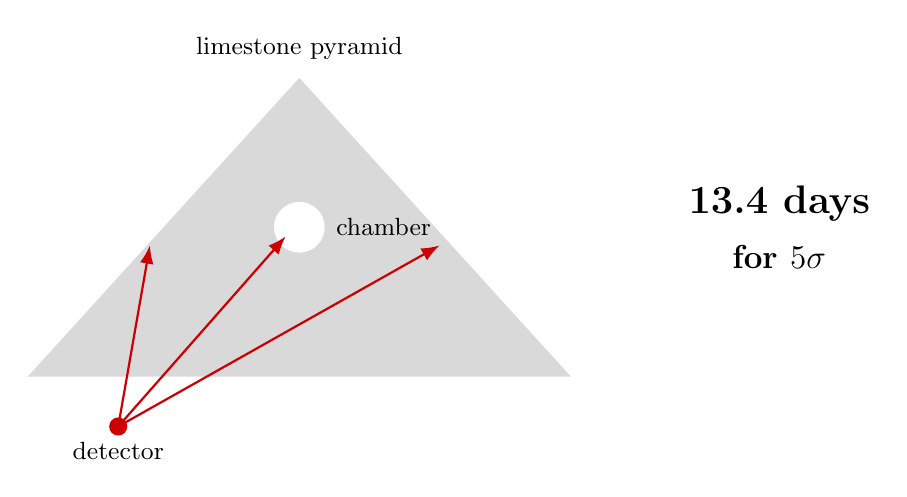
\begin{tikzpicture}[scale=1.15,>=Latex]
  \fill[gray!30] (0,0) -- (3.0,3.3) -- (6.0,0) -- cycle;
  \fill[white] (3.0,1.65) circle (0.28);
  \fill[red!80!black] (1.0,-0.55) circle (0.10);
  \draw[red!80!black,thick,-{Latex}] (1.0,-0.55) -- (2.85,1.55);
  \draw[red!80!black,thick,-{Latex}] (1.0,-0.55) -- (1.35,1.45);
  \draw[red!80!black,thick,-{Latex}] (1.0,-0.55) -- (4.55,1.45);
  \node[below] at (1.0,-0.62) {\small detector};
  \node[above] at (3.0,3.4) {\small limestone pyramid};
  \node[right] at (3.3,1.65) {\small chamber};
  \node[align=center,font=\bfseries\Large] at (8.3,1.65) {13.4 days\\[2pt]
    \large for $5\sigma$};
\end{tikzpicture}
\end{center}
\spoken
Good morning. Our project asks how long a small muon detector must run before
it can see a hidden chamber inside a solid limestone pyramid. The answer under
our baseline model is 13.4 days for a five-sigma expected signal, and 4.8 days
for three sigma. I will show why muons can do this, how the simulation works,
how we separate signal from noise, and what changes the answer.
\end{slidebox}

\newpage
\begin{slidebox}{2}{Why muons can see through rock}{1:20}
\onslide
\begin{itemize}
  \item Cosmic-ray protons make pions; pions decay into muons.
  \item Muon: heavy electron, 207$m_e$, lifetime 2.2~$\mu$s, dilated by
        $\gamma$.
  \item Flux: $10^4$~m$^{-2}$~min$^{-1}$ at sea level.
  \item Energy loss: $a+bE$; 2~MeV per g/cm$^2$; 100~m limestone needs
        52.6~GeV.
  \item Muons survive because radiative loss scales as $1/m^2$.
\end{itemize}
\figlabel two large TikZ panels: (left) atmosphere shower and muon paths;
(right) ionisation and radiative energy-loss curves with the MIP marked.
\begin{center}
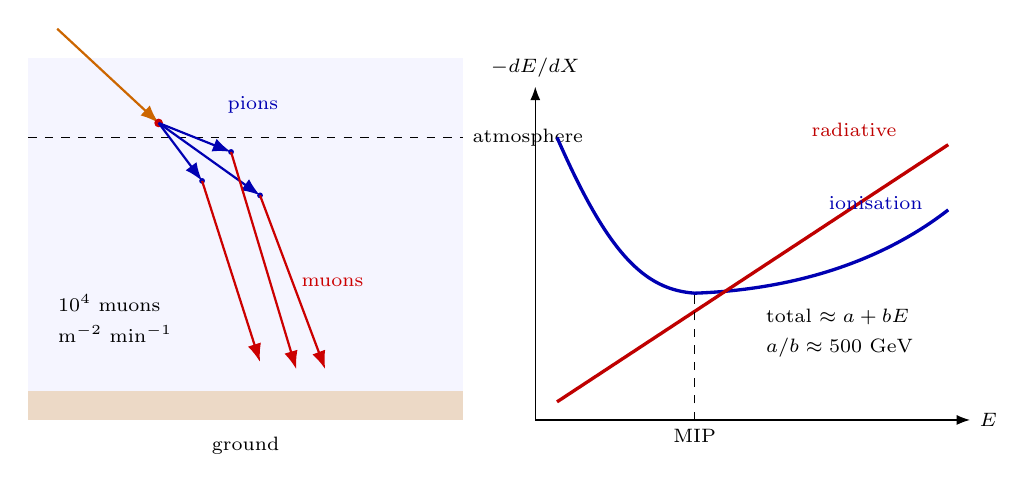
\begin{tikzpicture}[scale=0.92,>=Latex]
  % atmosphere panel
  \fill[blue!4] (0,0) rectangle (6.0,5.0);
  \fill[brown!30] (0,0) rectangle (6.0,0.4);
  \draw[dashed] (0,3.9) -- (6.0,3.9);
  \node[right] at (6.0,3.9) {\scriptsize atmosphere};
  \draw[thick,orange!80!black,-{Latex}] (0.4,5.4) -- (1.8,4.1);
  \fill[red!80!black] (1.8,4.1) circle (0.06);
  \foreach \x/\y in {2.4/3.3, 2.8/3.7, 3.2/3.1} {
    \draw[blue!70!black,thick,-{Latex}] (1.8,4.1) -- (\x,\y);
    \fill[blue!70!black] (\x,\y) circle (0.04);
  }
  \draw[red!80!black,thick,-{Latex}] (2.4,3.3) -- (3.2,0.8);
  \draw[red!80!black,thick,-{Latex}] (2.8,3.7) -- (3.7,0.7);
  \draw[red!80!black,thick,-{Latex}] (3.2,3.1) -- (4.1,0.7);
  \node[blue!70!black] at (3.1,4.35) {\scriptsize pions};
  \node[red!80!black] at (4.2,1.9) {\scriptsize muons};
  \node[align=left] at (1.2,1.4)
    {\scriptsize $10^4$ muons\\[-1pt]\scriptsize m$^{-2}$ min$^{-1}$};
  \node at (3.0,-0.35) {\scriptsize ground};
  % energy loss panel
  \begin{scope}[shift={(7.0,0.0)}]
    \draw[->] (0,0) -- (6.0,0) node[right] {\scriptsize $E$};
    \draw[->] (0,0) -- (0,4.6) node[above] {\scriptsize $-dE/dX$};
    \draw[very thick,blue!70!black] (0.3,3.9) .. controls (1.0,2.3)
      and (1.5,1.8) .. (2.2,1.75) .. controls (3.6,1.8) and (4.8,2.2)
      .. (5.7,2.9);
    \draw[very thick,red!75!black] (0.3,0.25) -- (5.7,3.8);
    \draw[dashed] (2.2,0) -- (2.2,1.75);
    \node[below] at (2.2,0) {\scriptsize MIP};
    \node[blue!70!black] at (4.7,3.0) {\scriptsize ionisation};
    \node[red!75!black] at (4.4,4.0) {\scriptsize radiative};
    \node[align=left] at (4.2,1.2)
      {\scriptsize total $\approx a+bE$\\[-1pt]
       \scriptsize $a/b\approx500$~GeV};
  \end{scope}
\end{tikzpicture}
\end{center}
\spoken
A cosmic-ray proton hits a nucleus about 15 kilometres up and produces pions,
which decay into muons. A muon is a heavy electron: 207 times the electron
mass, same charge, two-point-two microseconds at rest. Naively it decays after
660 metres, but it reaches the ground because time is dilated by gamma.
Roughly ten thousand muons cross each square metre every minute. Why do they
penetrate? Energy loss has two pieces: ionisation, about 2 MeV per gram per
square centimetre, and radiative loss, which grows with energy. Radiative loss
scales as one over mass squared, so a muon radiates about 43,000 times less
readily than an electron. One hundred metres of limestone needs 52.6 GeV. Only
the high-energy tail gets through, and that tail is our beam.
\end{slidebox}

\newpage
\begin{slidebox}{3}{Muography, the question, and the baseline}{1:20}
\onslide
\begin{itemize}
  \item Opacity $\varrho=\int\rho\,d\ell$: less rock $\rightarrow$ more muons.
  \item One direction = one pixel; a 2D radiograph, not a 3D CT.
  \item Baseline: 230~m base, 139~m high, 10~m chamber, 0.25~m$^2$ detector,
        $\pm40^\circ$, $2^\circ$ pixels.
  \item Question: how many days for the \emph{expected} signal to reach
        $5\sigma$?
\end{itemize}
\figlabel left: large TikZ ray diagram through the pyramid; right: a compact
parameter table with the same numbers as the report.
\begin{center}
\begin{minipage}{0.57\linewidth}
\centering
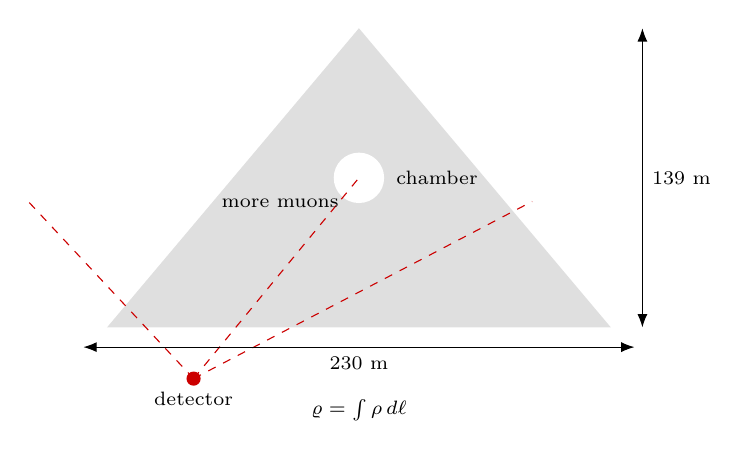
\begin{tikzpicture}[scale=1.0,>=Latex]
  \fill[gray!25] (0,0) -- (3.2,3.8) -- (6.4,0) -- cycle;
  \fill[white] (3.2,1.9) circle (0.32);
  \node[right] at (3.55,1.9) {\scriptsize chamber};
  \fill[red!80!black] (1.1,-0.65) circle (0.09);
  \node[below] at (1.1,-0.7) {\scriptsize detector};
  \draw[red!80!black,dashed] (1.1,-0.65) -- (-1.0,1.6);
  \draw[red!80!black,dashed] (1.1,-0.65) -- (3.2,1.9);
  \draw[red!80!black,dashed] (1.1,-0.65) -- (5.4,1.6);
  \node[above] at (2.2,1.4) {\scriptsize more muons};
  \draw[<->] (-0.3,-0.25) -- (6.7,-0.25)
    node[midway,below] {\scriptsize 230~m};
  \draw[<->] (6.8,0) -- (6.8,3.8) node[midway,right] {\scriptsize 139~m};
  \node at (3.2,-1.05) {\scriptsize $\varrho=\int\rho\,d\ell$};
\end{tikzpicture}
\end{minipage}\hfill
\begin{minipage}{0.39\linewidth}
\centering\small
\begin{tabular}{@{}ll@{}}
\toprule
Parameter & Value \\
\midrule
Base / height & 230 / 139~m \\
Chamber radius & 10~m \\
Chamber centre & $(0,0,70)$~m \\
Detector area & 0.25~m$^2$ \\
Detector position & $(0,-40,3)$~m \\
Field / bin & $\pm40^\circ$ / $2^\circ$ \\
Pixels & 1681 \\
Ray step & 0.25~m \\
Seed & 0 \\
\bottomrule
\end{tabular}
\end{minipage}
\end{center}
\spoken
Muography turns that beam into an image. Along each direction we integrate the
density: that is the opacity. More rock means fewer surviving muons, so a void
shows up as an excess. One direction becomes one pixel; this is a radiograph,
not a full three-dimensional tomography. Our baseline is a 230 metre square
pyramid, 139 metres high, with a 10 metre spherical chamber at height 70. The
detector is a quarter square metre at minus 40 metres, with a plus or minus 40
degree field and two degree pixels, 1681 directions. The research question is
the number on the previous slide: how many days before the expected signal
reaches five sigma?
\end{slidebox}


\newpage
\begin{slidebox}{4}{The five-step method, and the data it produces}{1:25}
\onslide
\begin{itemize}
  \item Density field $\rightarrow$ ray march $\rightarrow$ expected counts
        $\rightarrow$ noise/ratio $\rightarrow$ significance/scan.
  \item Two targets: chamber and filled-solid twin; their ratio removes the
        pyramid.
  \item Shared module \texttt{opacity\_map}, \texttt{expected\_counts};
        seed 0; fresh kernel.
  \item Data: 1681-pixel maps, 500 null runs, 500 void runs, six one-parameter
        scans.
\end{itemize}
\figlabel a large horizontal pipeline with icons and a data-structure inset
showing the $41\times41$ map, the angle grids, and the two twin branches.
\begin{center}
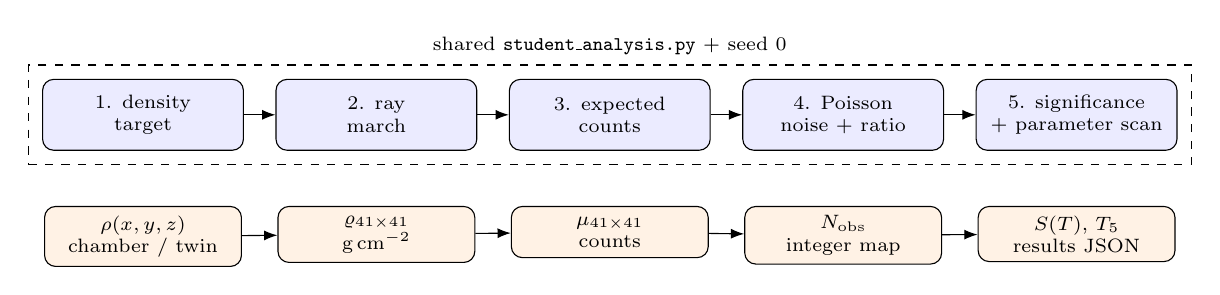
\begin{tikzpicture}[node distance=4mm,>=Latex,
  box/.style={draw,rounded corners,fill=blue!8,align=center,
              minimum width=2.55cm,minimum height=0.9cm,font=\scriptsize},
  data/.style={draw,fill=orange!10,align=center,rounded corners,
               minimum width=2.5cm,minimum height=0.65cm,font=\scriptsize}]
  \node[box] (t) {1. density\\target};
  \node[box,right=of t] (r) {2. ray\\march};
  \node[box,right=of r] (c) {3. expected\\counts};
  \node[box,right=of c] (n) {4. Poisson\\noise + ratio};
  \node[box,right=of n] (s) {5. significance\\+ parameter scan};
  \draw[->] (t) -- (r);
  \draw[->] (r) -- (c);
  \draw[->] (c) -- (n);
  \draw[->] (n) -- (s);
  \node[data,below=7mm of t] (d1) {$\rho(x,y,z)$\\chamber / twin};
  \node[data,below=7mm of r] (d2) {$\varrho_{41\times41}$\\g\,cm$^{-2}$};
  \node[data,below=7mm of c] (d3) {$\mu_{41\times41}$\\counts};
  \node[data,below=7mm of n] (d4) {$N_{\rm obs}$\\integer map};
  \node[data,below=7mm of s] (d5) {$S(T)$, $T_5$\\results JSON};
  \draw[->] (d1) -- (d2);
  \draw[->] (d2) -- (d3);
  \draw[->] (d3) -- (d4);
  \draw[->] (d4) -- (d5);
  \node[draw,dashed,fit=(t)(r)(c)(n)(s),inner sep=5pt,
        label={[font=\scriptsize]above:shared \texttt{student\_analysis.py} + seed 0}] {};
\end{tikzpicture}
\end{center}
\spoken
The method is five steps. Step one is a density function: rock, air, or a
chamber. Step two is pure geometry: march a ray through every direction and add
density times length. Step three converts opacity to a minimum energy and then
to expected muon counts. Step four draws Poisson noise and divides by the
no-void twin. Step five builds the significance map and scans one parameter at
a time. The important engineering choice is that steps two and three live in a
shared module, not in a notebook; every notebook imports the same functions and
uses seed zero. The data products are the 1681-pixel maps, 500 null runs, 500
chamber runs, and six one-parameter scans.
\end{slidebox}

\newpage
\begin{slidebox}{5}{Ray tracing: from geometry to an opacity map}{1:20}
\onslide
\begin{itemize}
  \item Tangent-plane camera; 1681 rays; 0.25~m steps.
  \item Chamber notch: 4,935~g/cm$^2$, against the geometric 5,000.
  \item Ray-step halving changes the map by $\le0.24\%$.
  \item No-void control is zero away from the chamber.
\end{itemize}
\figlabel left: the density slice; right: a TikZ camera-grid showing the
$41\times41$ directions and one highlighted signal ray at $30.8^\circ$.
\begin{center}
\begin{minipage}{0.55\linewidth}
\centering
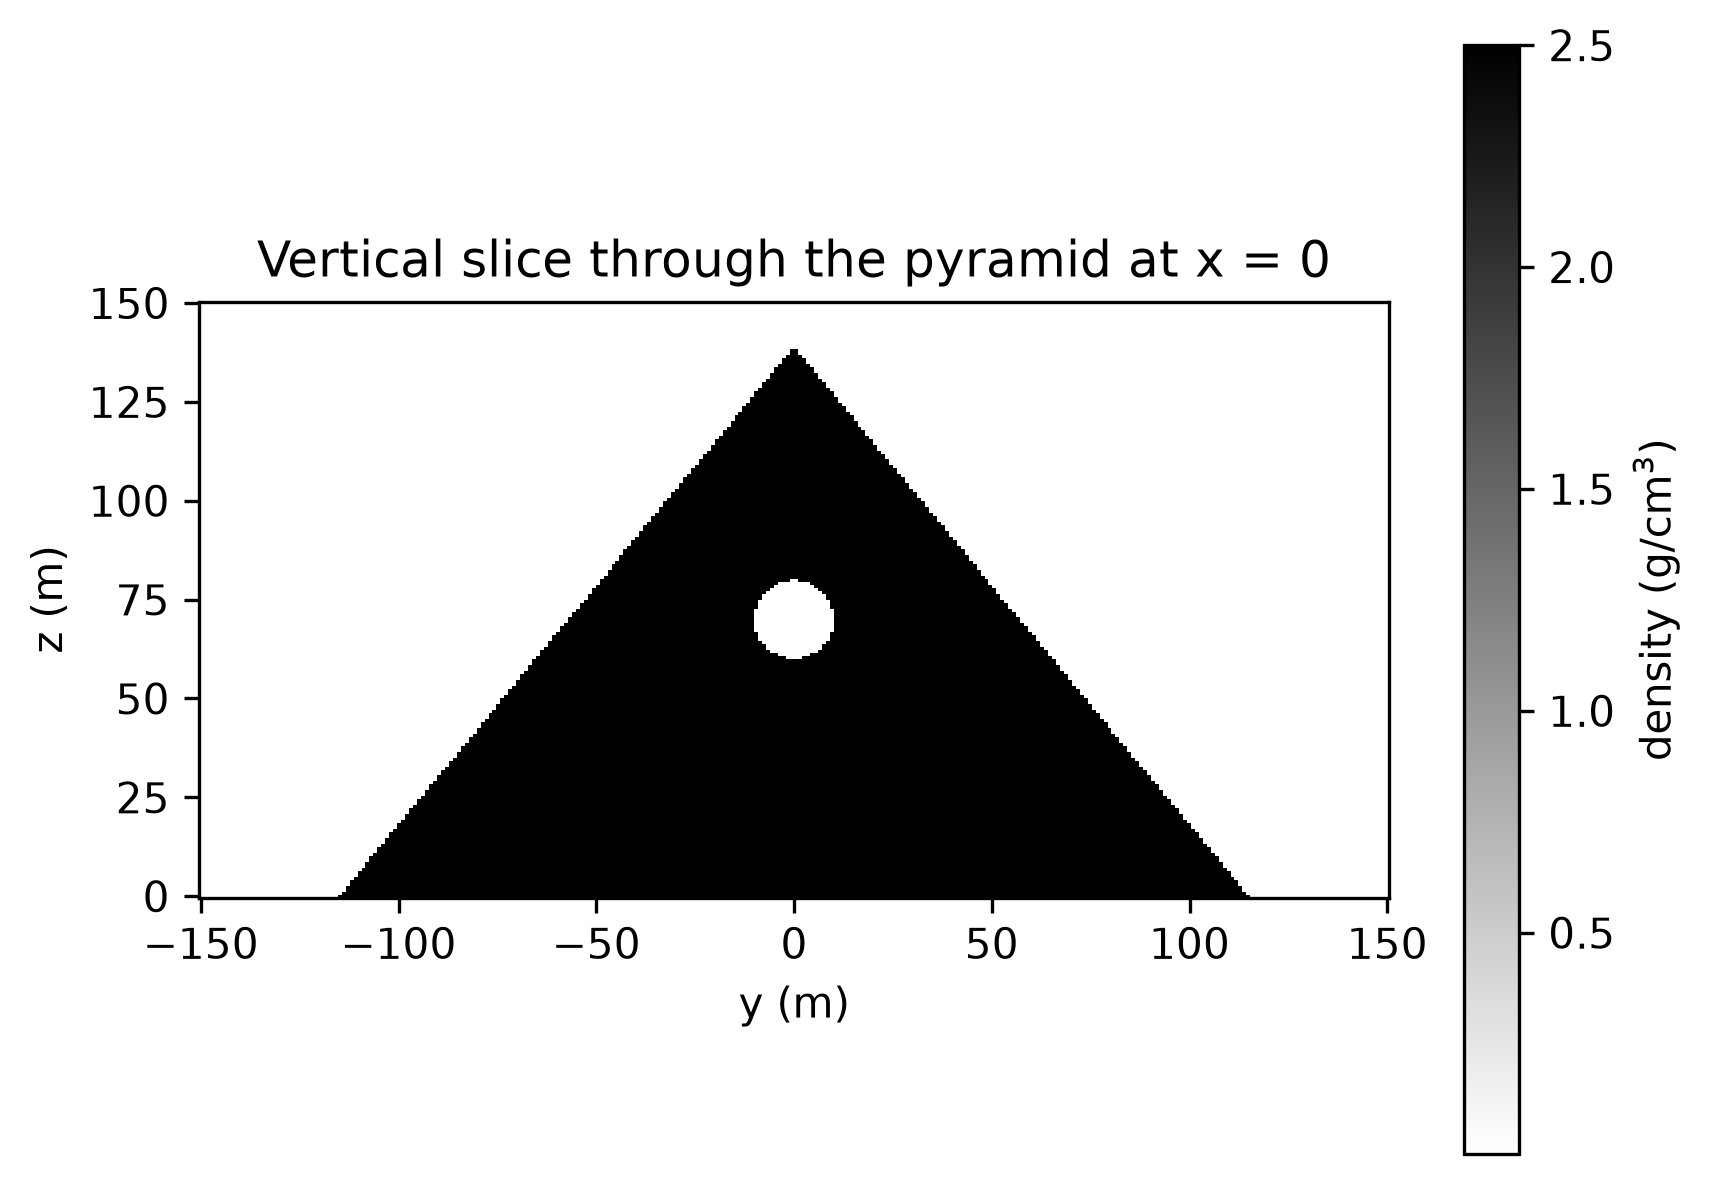
\includegraphics[width=\linewidth]{05_density_slice.png}
\end{minipage}\hfill
\begin{minipage}{0.42\linewidth}
\centering
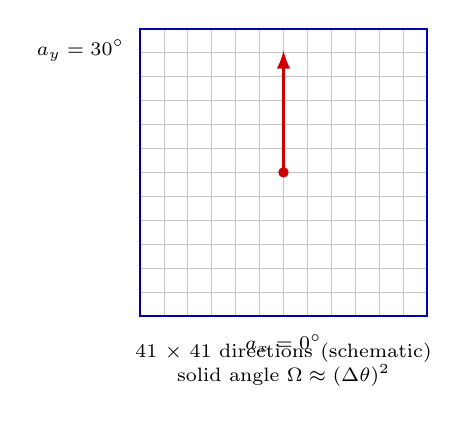
\begin{tikzpicture}[scale=0.95,>=Latex]
  \draw[step=0.32cm,gray!45,very thin] (0,0) grid (3.84,3.84);
  \draw[thick,blue!70!black] (0,0) rectangle (3.84,3.84);
  \fill[red!80!black] (1.92,1.92) circle (0.07);
  \draw[red!80!black,thick,-{Latex}] (1.92,1.92) -- (1.92,3.55);
  \node[below] at (1.92,-0.12) {\scriptsize $a_x=0^\circ$};
  \node[left] at (-0.08,3.55) {\scriptsize $a_y=30^\circ$};
  \node[align=center,font=\scriptsize] at (1.92,-0.65)
    {41 $\times$ 41 directions (schematic)\\[1pt]
     solid angle $\Omega\approx(\Delta\theta)^2$};
\end{tikzpicture}
\end{minipage}
\end{center}
\spoken
This is the geometry step. The camera is a tangent plane, so a direction is
two small angles. We trace 1681 rays in quarter-metre steps and add density
times length. The chamber is a 10 metre sphere, so the longest chord is 20
metres and the missing opacity should be 5,000 gram per square centimetre. We
measure 4,935, 1.3 per cent lower because the discrete ray misses the centre.
Halving the step changes the map by at most 0.24 per cent, and the no-void
control is flat away from the chamber. Those two checks are what convince us
the geometry is right before any statistics.
\end{slidebox}


\newpage
\begin{slidebox}{6}{Counts and reconstruction: the before/after image}{1:25}
\onslide
\begin{itemize}
  \item Raw counts: 191--1,197 per pixel, factor 6.3; the pyramid dominates.
  \item Twin target ratio: 1.0000 away, 1.4758 at the chamber.
  \item Peak: 366.8 with / 248.5 without; excess 118.3 muons in 30 days;
        $7.50\sigma$.
  \item Before: density slice. After: clean ratio. Both are needed.
\end{itemize}
\figlabel two large figures side by side: expected-count map and clean ratio
map with profile. Point at the axes before interpreting.
\begin{center}
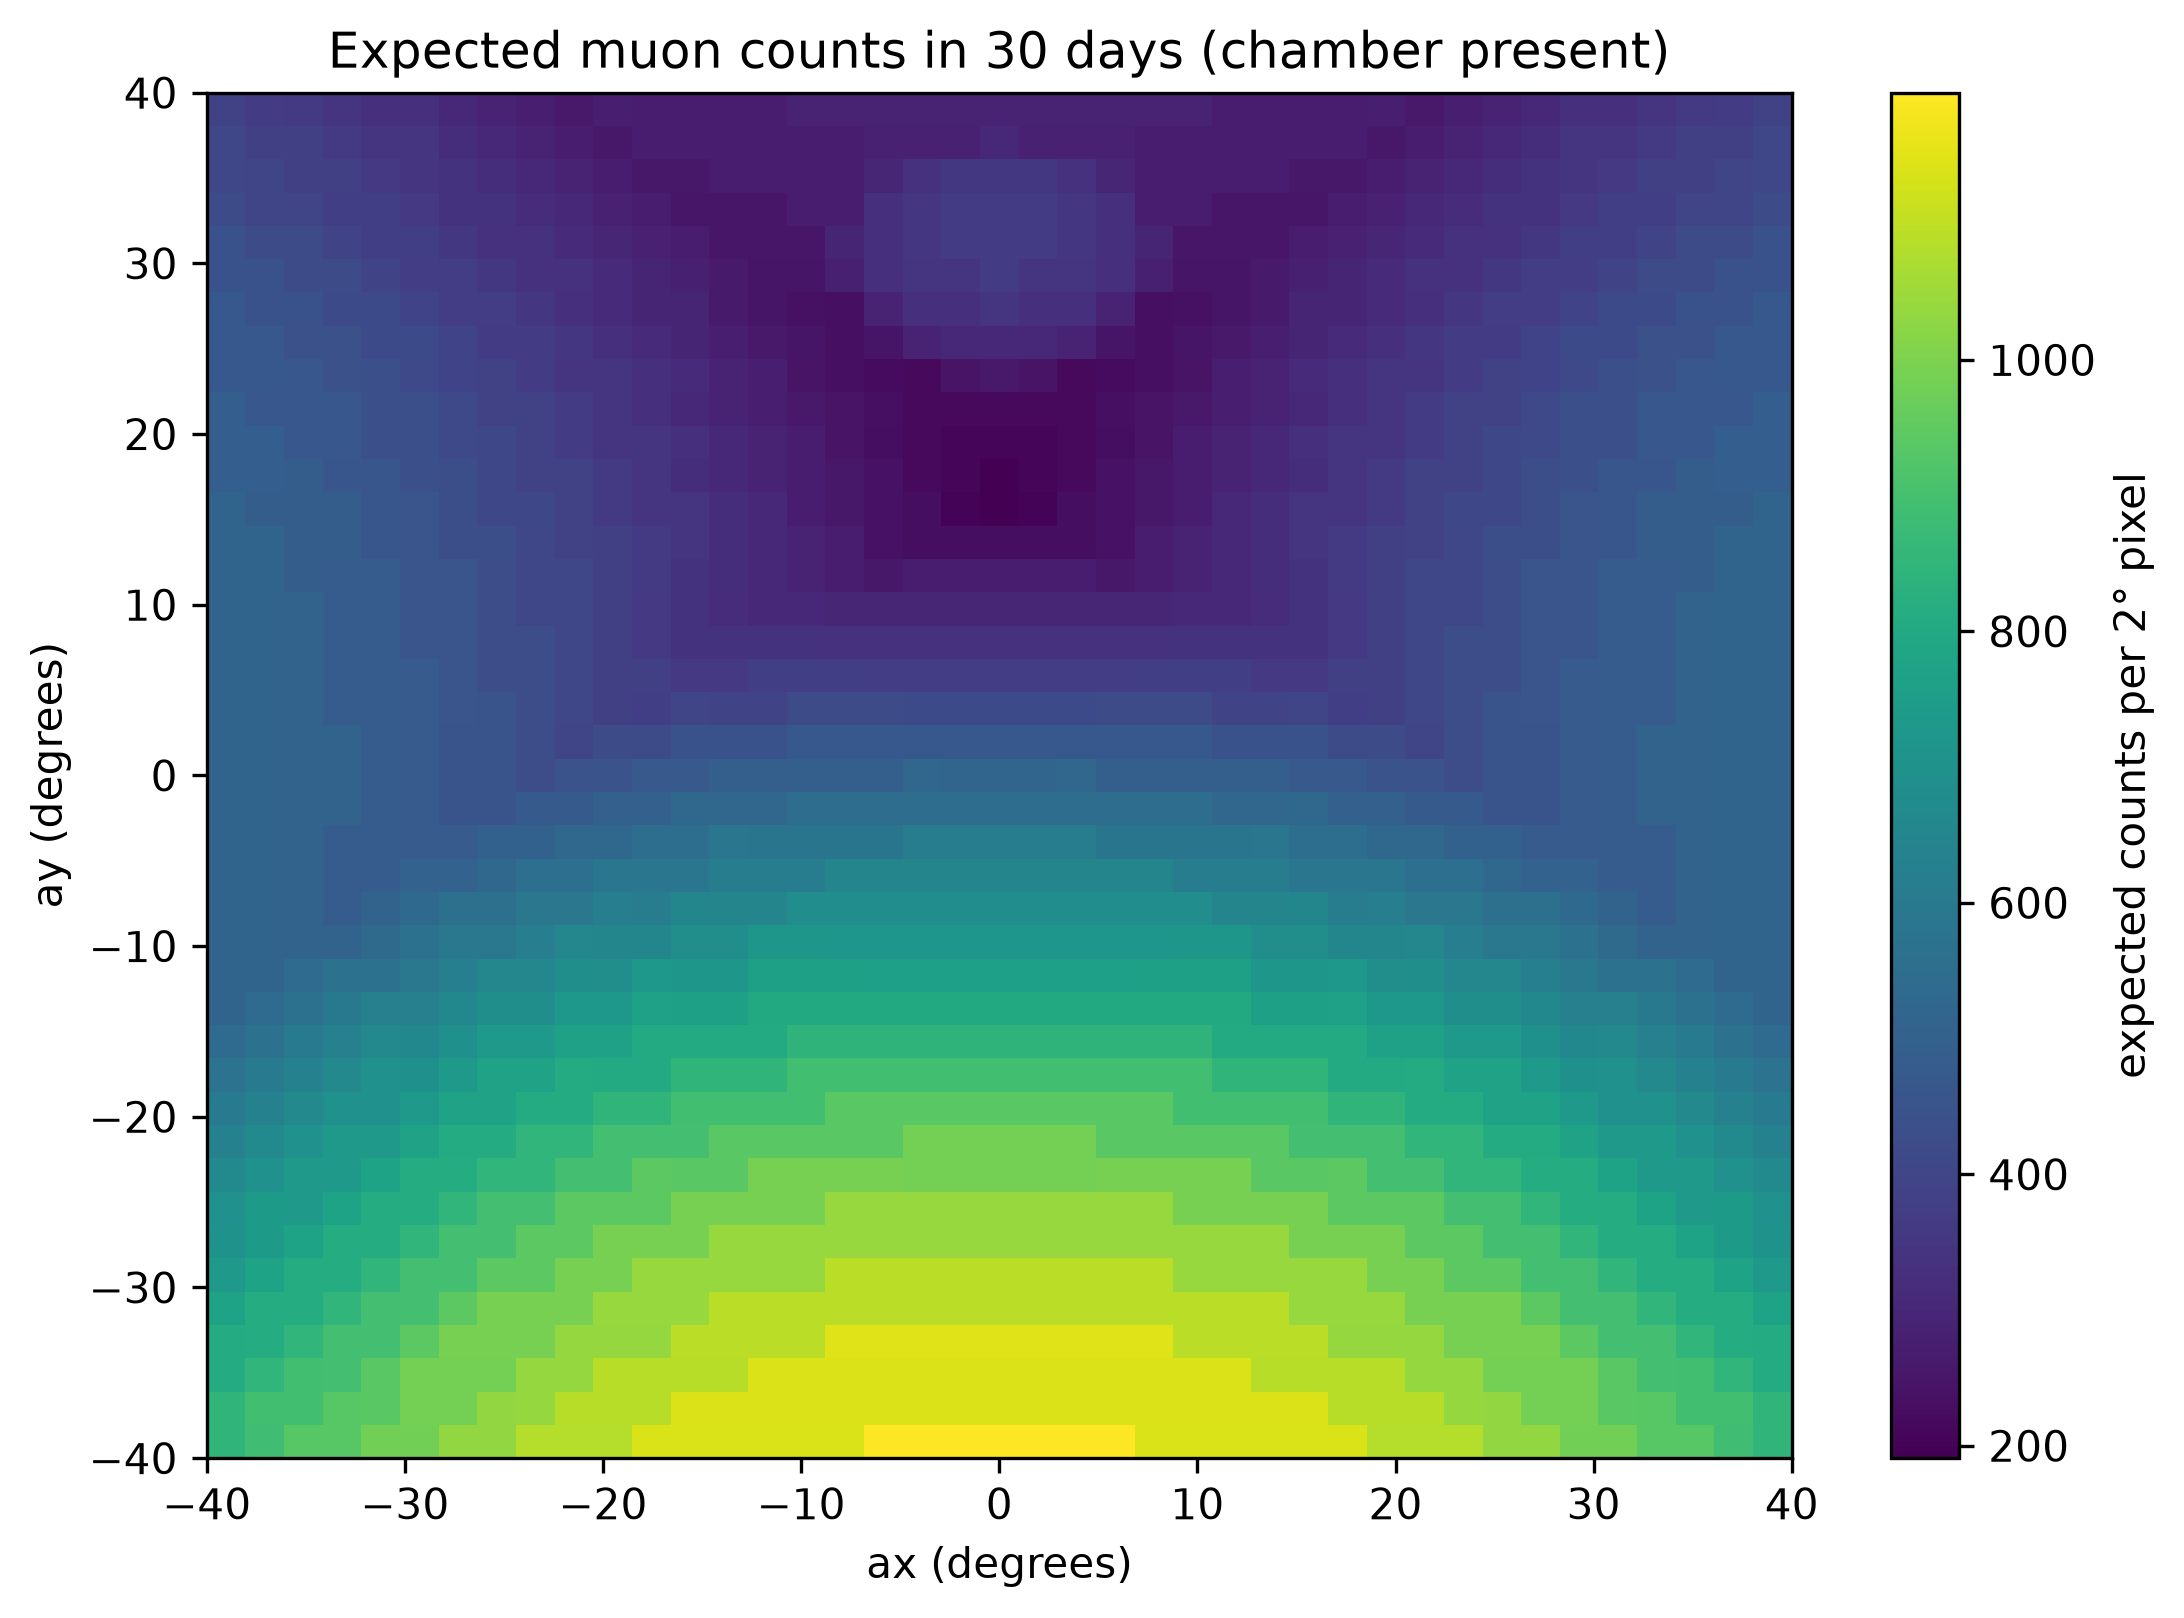
\includegraphics[width=0.47\linewidth]{08_expected_counts.png}\hfill
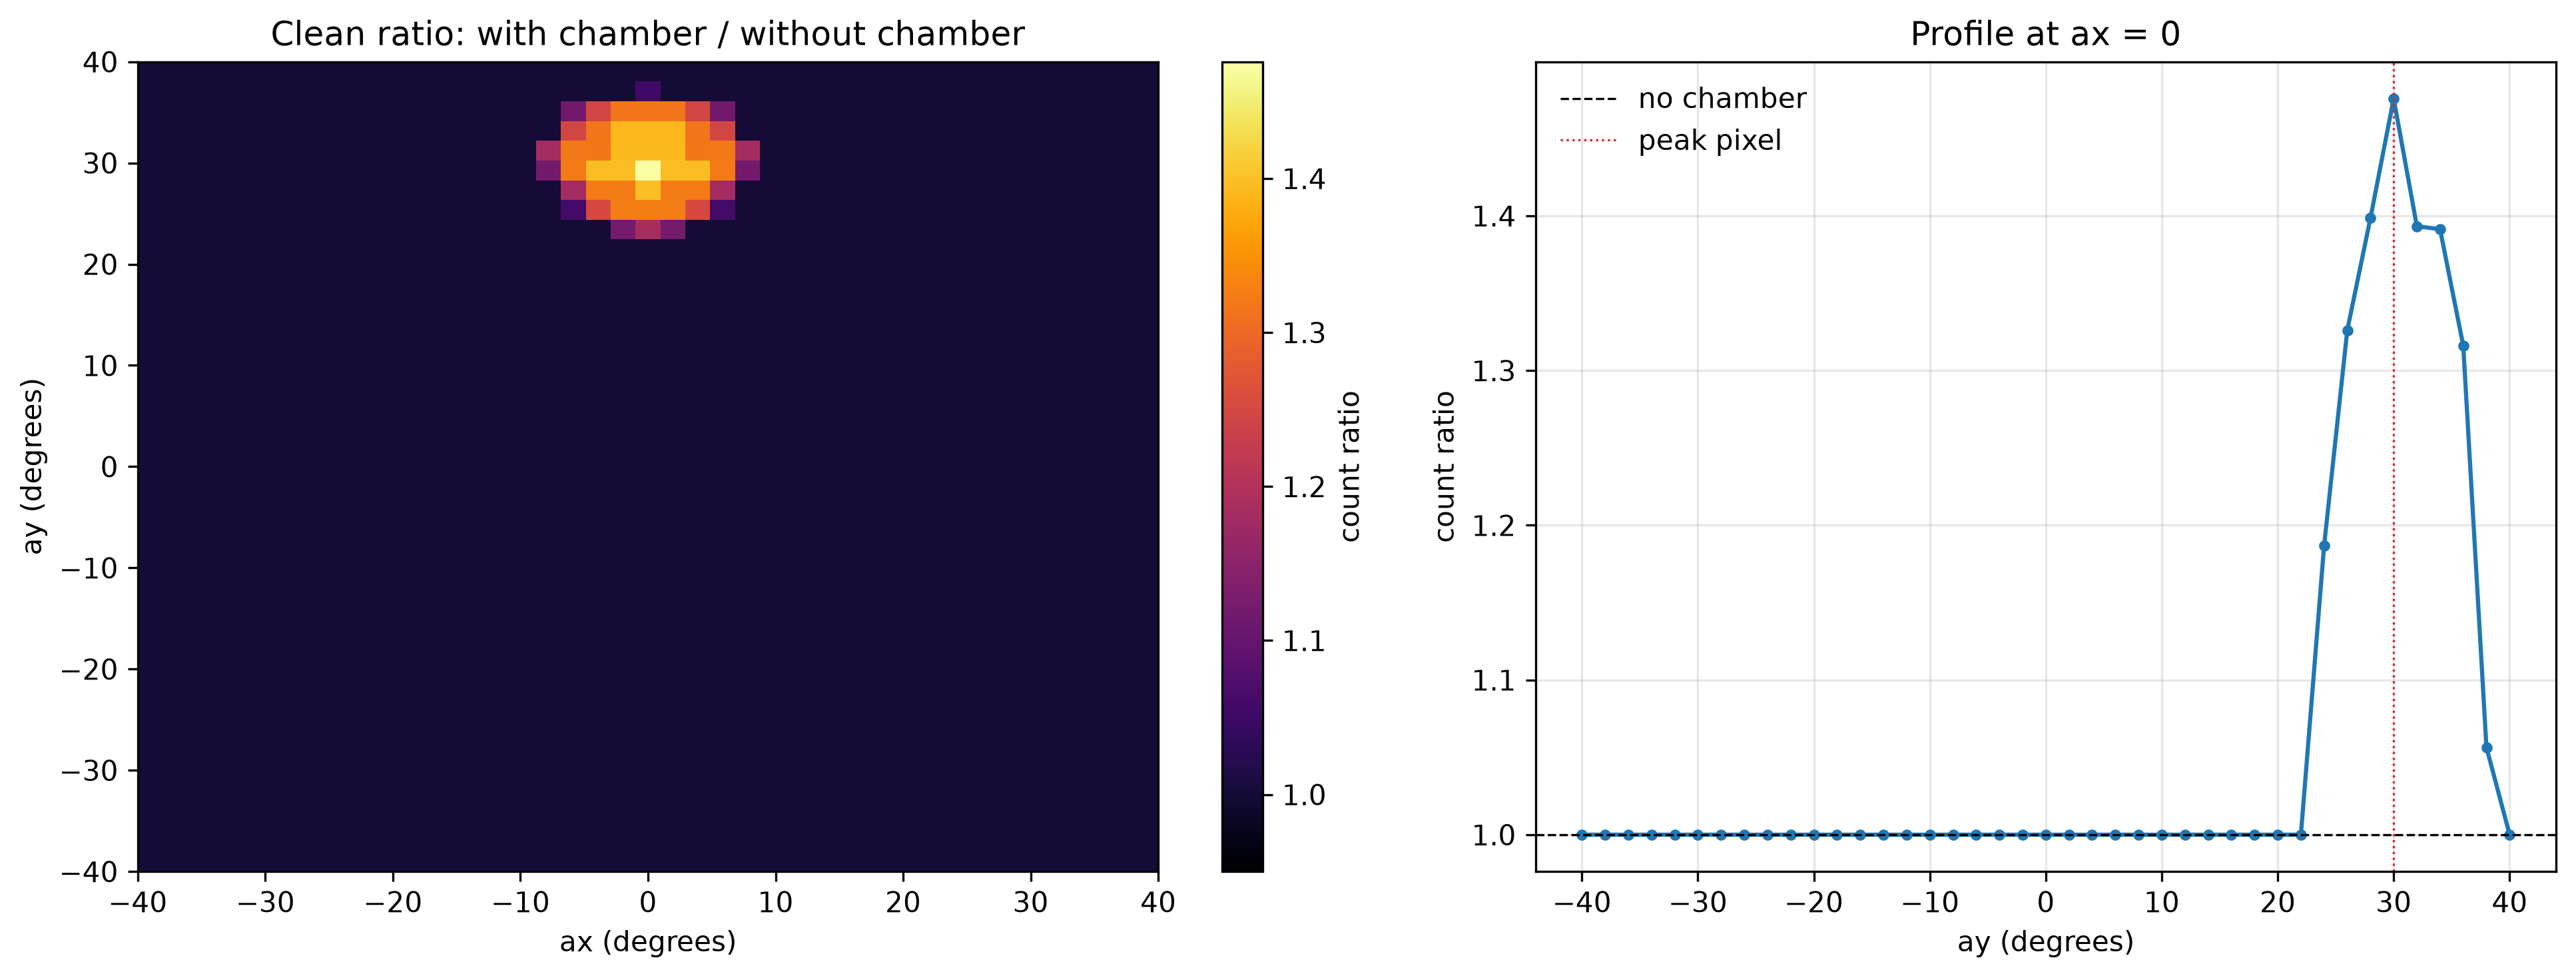
\includegraphics[width=0.50\linewidth]{09_clean_ratio.png}
\end{center}
\spoken
Step three gives counts, and step four gives the image. The raw 30-day map runs
from 191 to 1,197 counts per pixel, a factor 6.3, because the pyramid is thicker
in some directions. The chamber changes the total by only 0.36 per cent. So the
raw map is a picture of the pyramid, not the chamber. We build a twin target
with the chamber filled solid and divide. Away from the chamber the ratio is
1.0000 to four decimals. At the chamber it peaks at 1.4758: 366.8 counts with
the chamber, 248.5 without, an excess of 118 muons in 30 days, which is 7.50
sigma expected. This ratio map is the after image. The density slice is the
before image, and the gap between them is the whole point.
\end{slidebox}

\newpage
\begin{slidebox}{7}{Noise, significance, and the look-elsewhere effect}{1:30}
\onslide
\begin{itemize}
  \item Poisson: mean $\mu$, spread $\sqrt{\mu}$.
  \item Observed $S_{\rm obs}=(N-\mu_0)/\sqrt{\mu_0}$; expected
        $S_{\rm exp}=(\mu_{\rm void}-\mu_{\rm rock})/\sqrt{\mu_{\rm rock}}$.
  \item $S_{\rm exp}\propto\sqrt{T}$; fix one signal pixel once.
  \item 1681 pixels: null maximum is $3.44\sigma$ on average; 91.6\% of null
        maps have a $3\sigma$ pixel.
\end{itemize}
\figlabel left: Poisson bar sketch; right: null ensemble figure with maximum
and fixed-pixel distributions.
\begin{center}
\begin{minipage}{0.40\linewidth}
\centering
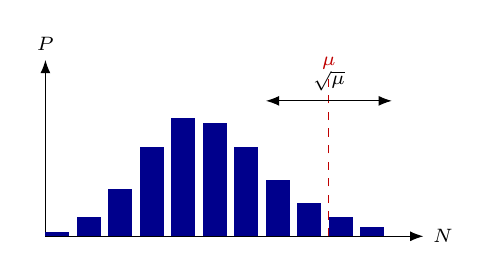
\begin{tikzpicture}[scale=0.80,>=Latex]
  \draw[->] (0,0) -- (6.0,0) node[right] {\scriptsize $N$};
  \draw[->] (0,0) -- (0,2.8) node[above] {\scriptsize $P$};
  \foreach \k/\h in {0/0.1,1/0.4,2/1.0,3/1.9,4/2.5,5/2.4,6/1.9,7/1.2,
                     8/0.7,9/0.4,10/0.2} {
    \fill[blue!55!black] (\k*0.5,0) rectangle ++(0.38,\h*0.75);
  }
  \draw[dashed,red!75!black] (4.5,0) -- (4.5,2.5);
  \node[red!75!black,above] at (4.5,2.5) {\scriptsize $\mu$};
  \draw[<->] (3.5,2.15) -- (5.5,2.15) node[midway,above] {\scriptsize $\sqrt{\mu}$};
\end{tikzpicture}
\end{minipage}\hfill
\begin{minipage}{0.57\linewidth}
\centering
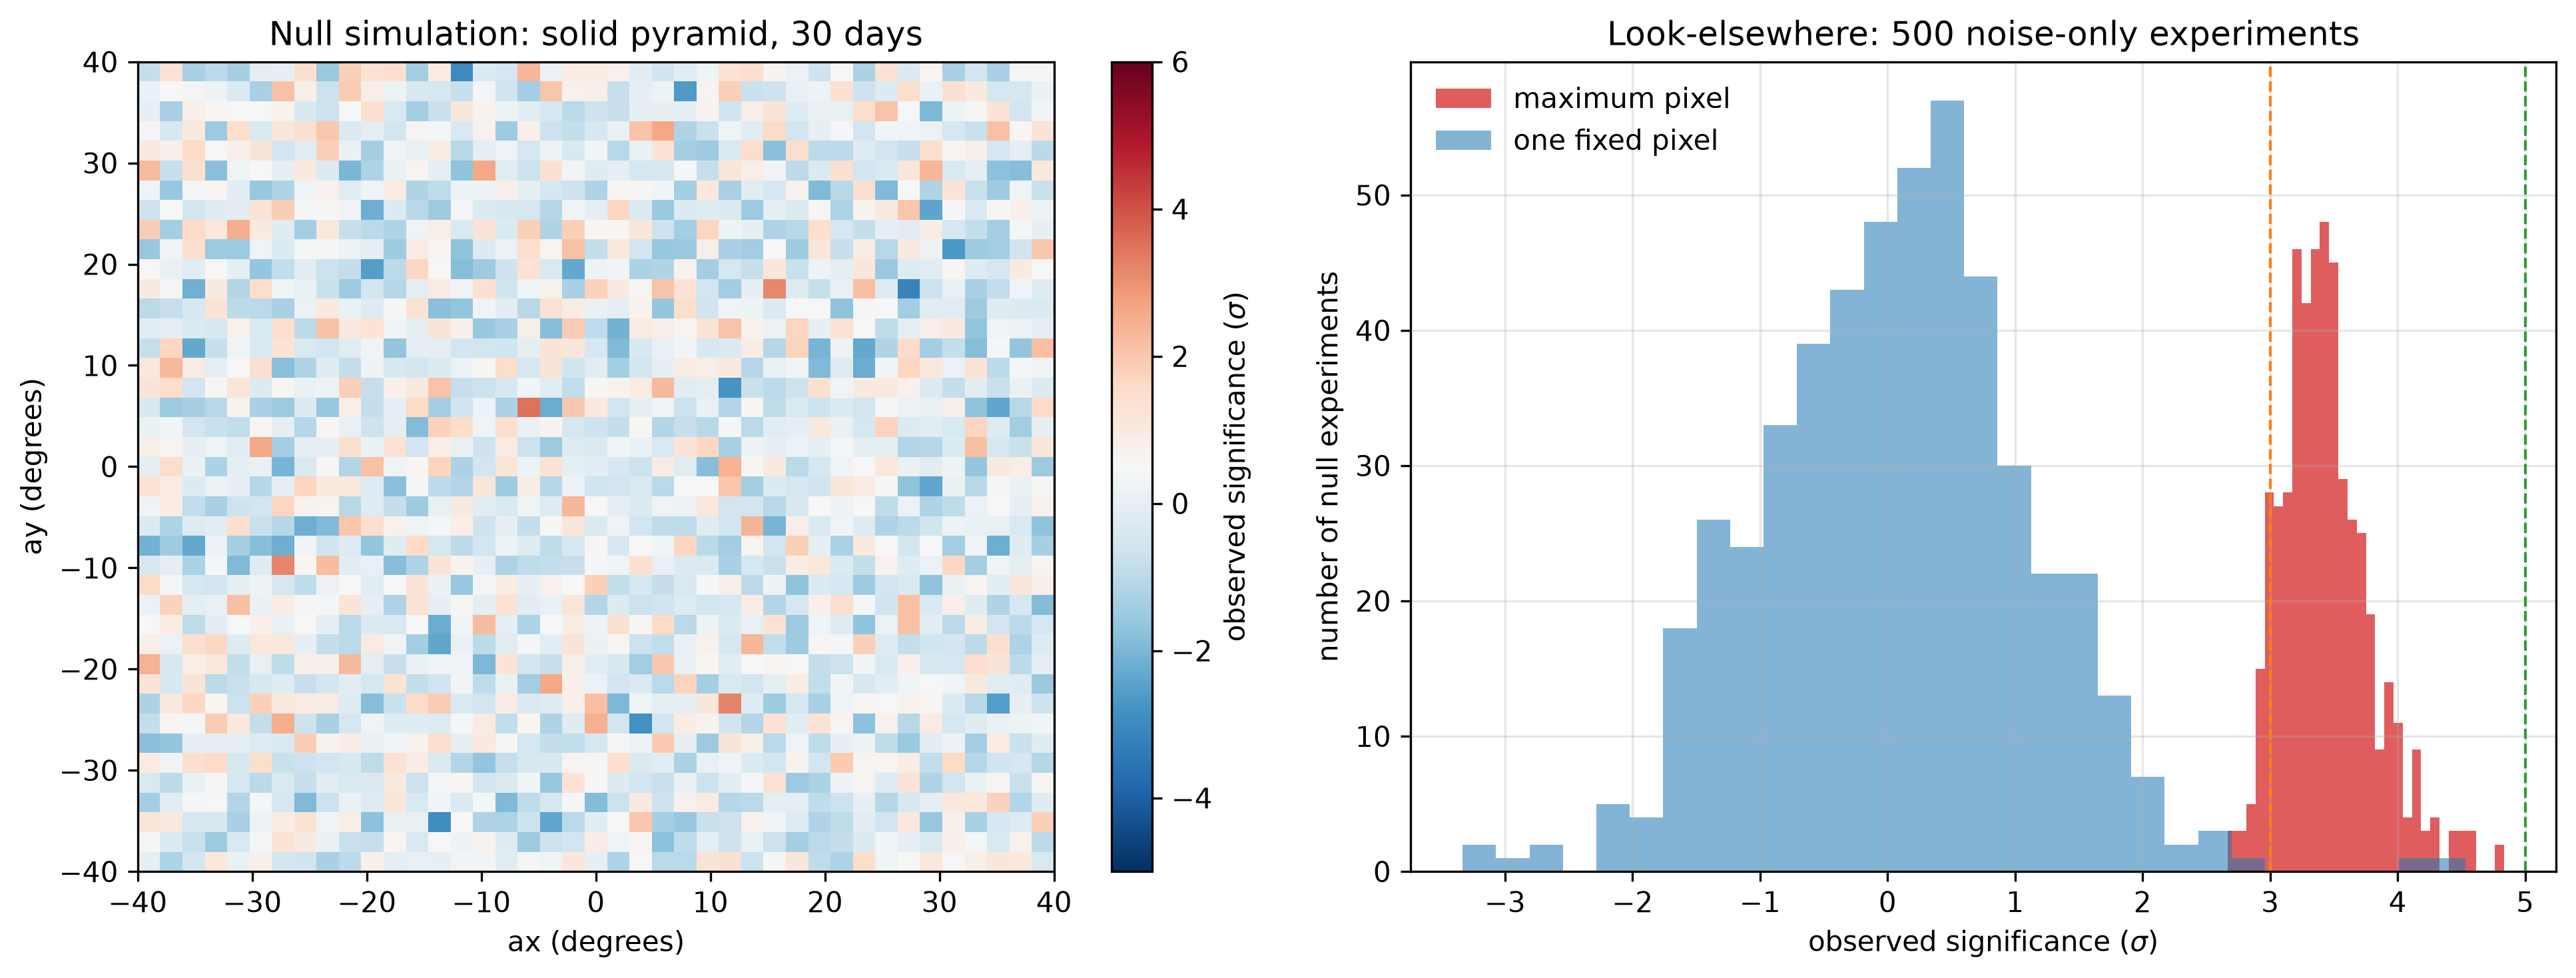
\includegraphics[width=\linewidth]{12_null_ensemble.png}
\end{minipage}
\end{center}
\spoken
Now the statistics. A measurement is a Poisson draw: mean mu, spread root mu.
Observed significance uses one noisy count and changes with the seed. Expected
significance uses the two expectation maps and is deterministic. Because both
signal and background grow with time, expected significance grows as root T.
We choose one signal pixel from the noiseless maps and never move it. Why is
that necessary? The null figure on the right: 500 solid-pyramid runs. One fixed
pixel has mean zero and standard deviation one, as it should. The maximum over
1681 pixels has mean 3.44 sigma; 91.6 per cent of null maps contain a 3 sigma
pixel. A single 3 sigma pixel is not a discovery.
\end{slidebox}

\newpage
\begin{slidebox}{8}{The exposure curve and the headline}{1:30}
\onslide
\begin{itemize}
  \item Fixed pixel: $S=1.3696$ at 1 day; crosses $3\sigma$ at 4.82 days and
        $5\sigma$ at 13.4 days.
  \item 30 days: expected $7.50\sigma$; observed seed-0 value $7.70\sigma$.
  \item 200-run distributions: 14 days $5.12\pm1.24$ (54\% cross); 30 days
        $7.53\pm1.23$ (98\% cross).
  \item Deterministic benchmark, not a measurement.
\end{itemize}
\figlabel large exposure curve with the $3\sigma$/$5\sigma$ lines and the
observed points; a small definitions table in the corner.
\begin{center}
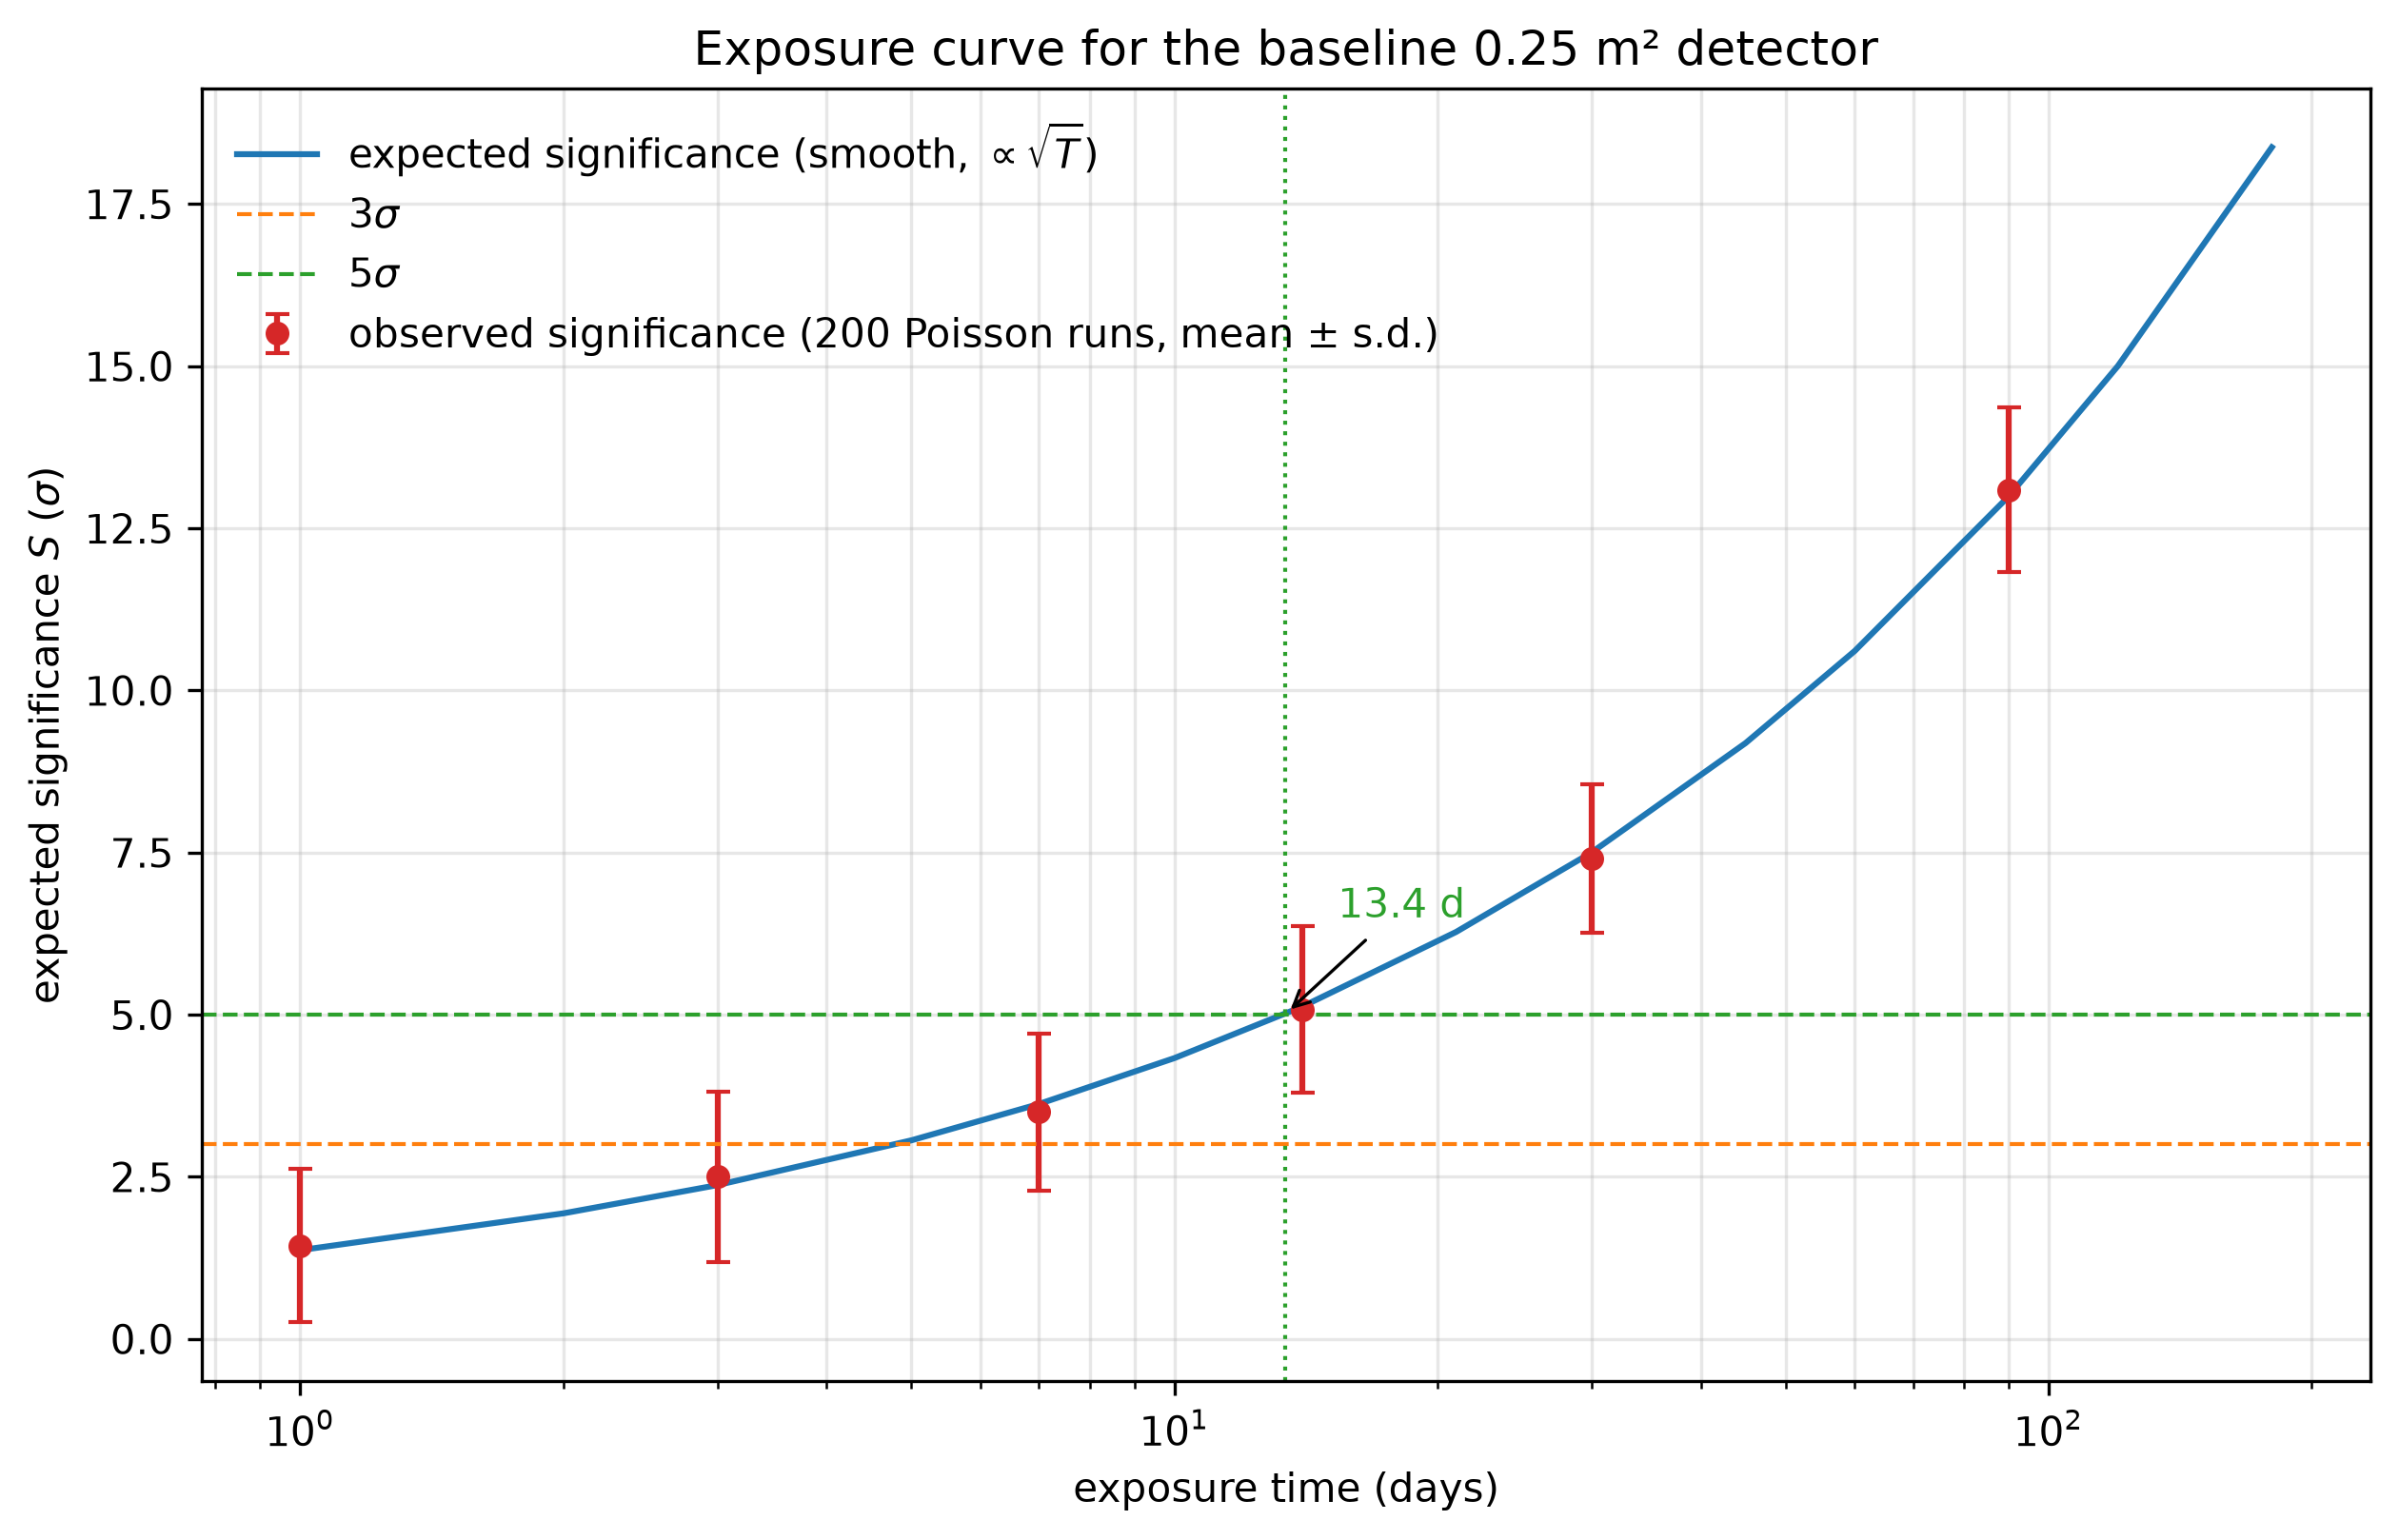
\includegraphics[width=0.72\linewidth]{11_exposure_curve.png}
\end{center}
\small
\begin{center}
\begin{tabular}{@{}lrr@{}}
\toprule
Definition & 30-day $S$ & $T_5$ (days) \\
\midrule
Peak pixel (official) & $7.50\sigma$ & 13.3 \\
Exact pixel solid angle & $6.98\sigma$ & 15.4 \\
Whole image (global) & $3.55\sigma$ & 59.5 \\
\bottomrule
\end{tabular}
\end{center}
\spoken
Here is the curve. At the fixed pixel, one day gives 1.3696 sigma. Three sigma
comes at 4.82 days; five sigma at 13.4. Thirty days gives 7.50 expected, and our
seed-zero observation gives 7.70. The red points are 200 runs at each exposure:
at 14 days the mean is 5.12 and 54 per cent cross five sigma; at 30 days it is
7.53 and 98 per cent cross. The number is deterministic, so it has no error bar.
The table shows the two alternative definitions: exact pixel solid angle gives
15.4 days, and whole-image global significance gives 59.5 days. Both are
reported, but the official headline is the per-pixel expected value.
\end{slidebox}


\newpage
\begin{slidebox}{9}{Study A: size, and Study B: depth}{1:25}
\onslide
\begin{itemize}
  \item A: $r=4$~m $\to$ 146.6 days; $r=20$~m $\to$ 1.99 days;
        $S\propto r^{1.32}$.
  \item The signal is the chord ($\propto r$), not the volume ($\propto r^3$).
  \item B: depth 55--110~m; $T_5$ 15.4 $\to$ 21.6 $\to$ 17.8 days.
  \item Shorter path competes with larger zenith angle; apex effect above 95~m.
\end{itemize}
\figlabel two large figures side by side: Study A size scaling and Study B
depth scaling.
\begin{center}
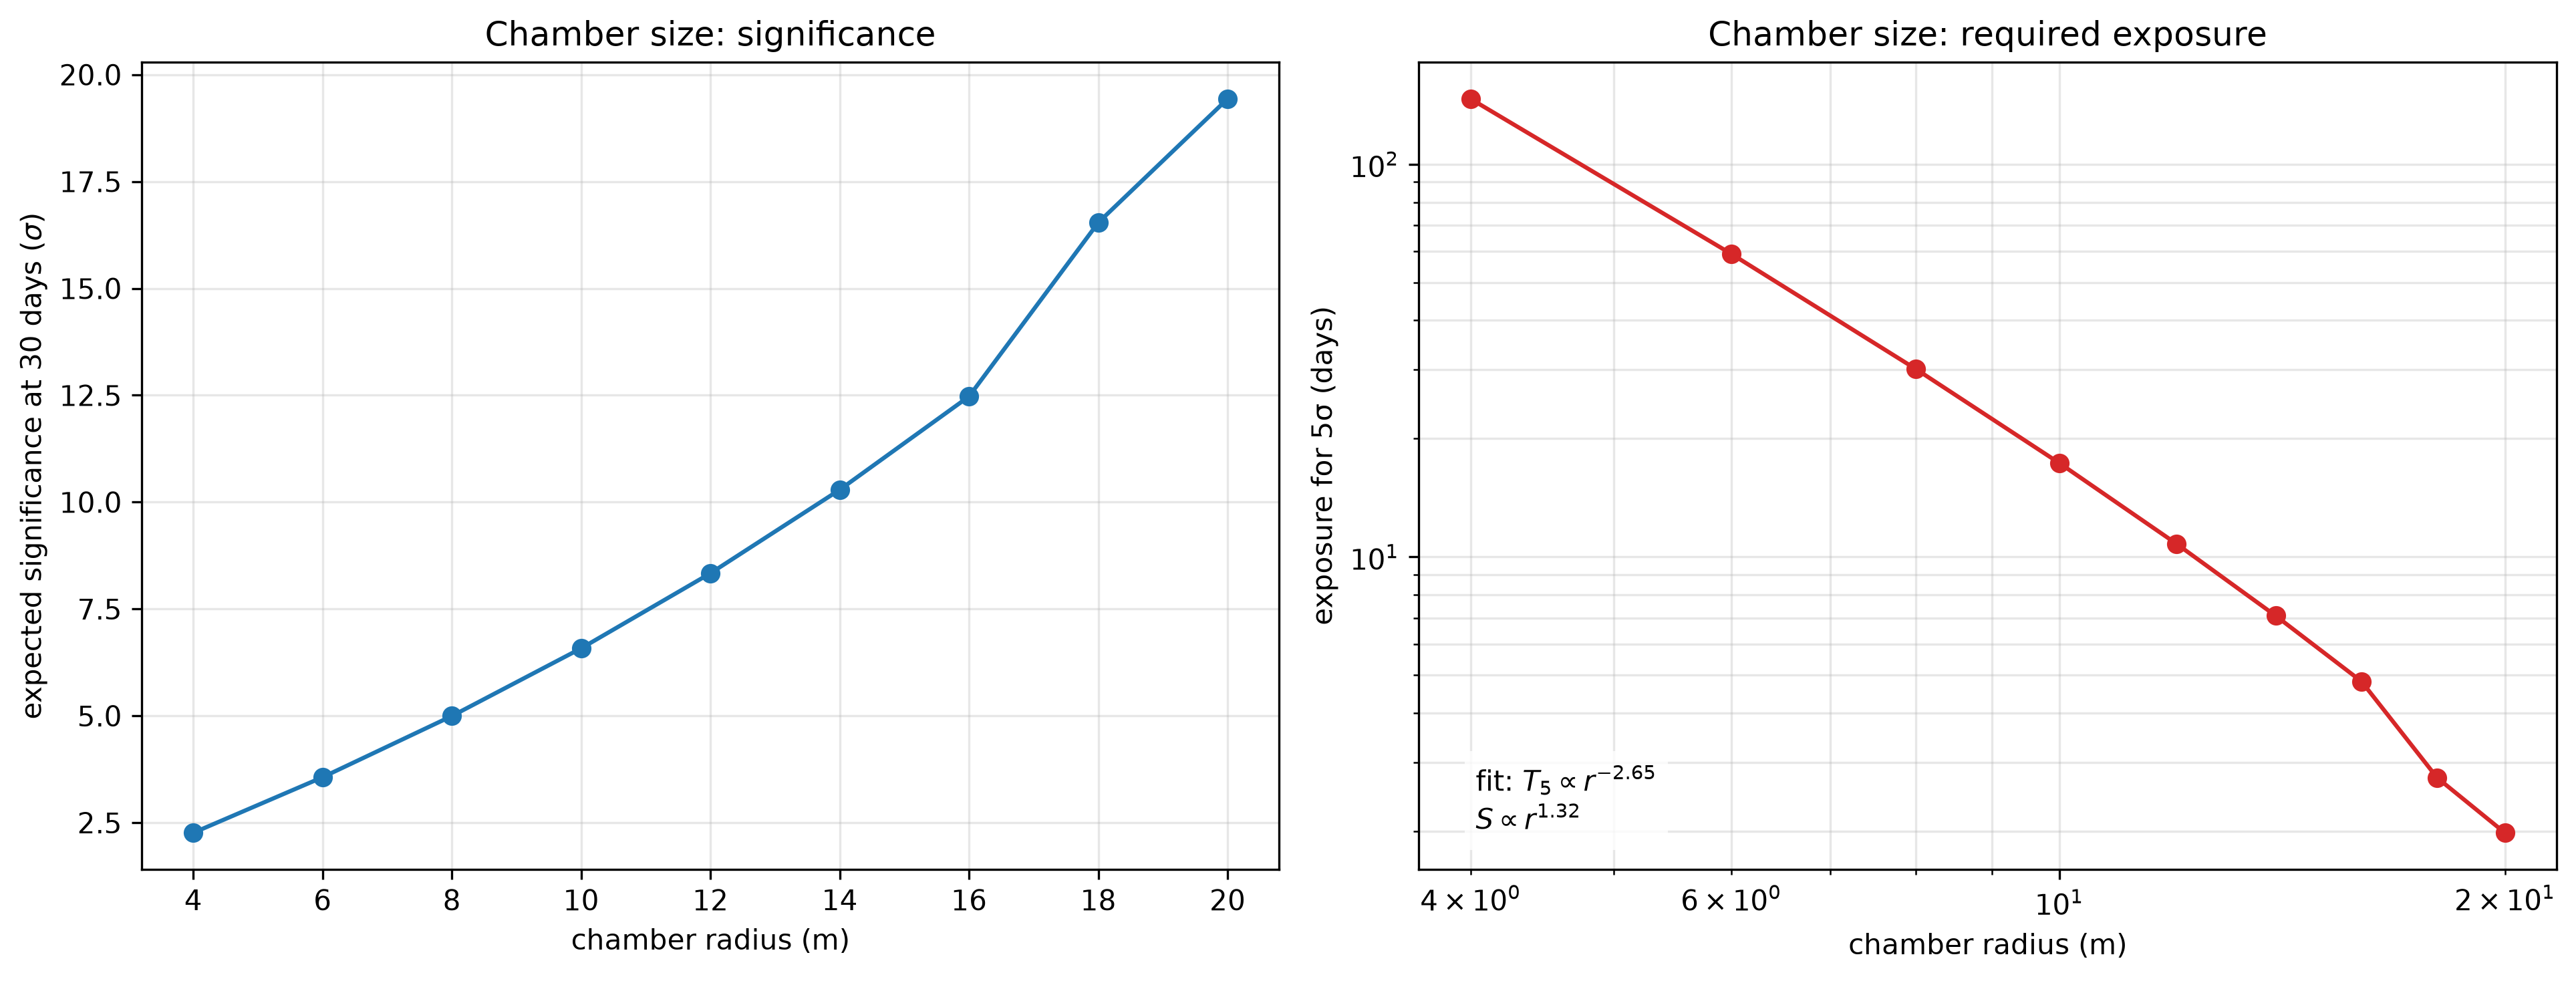
\includegraphics[width=0.49\linewidth]{14_study_A_size.png}\hfill
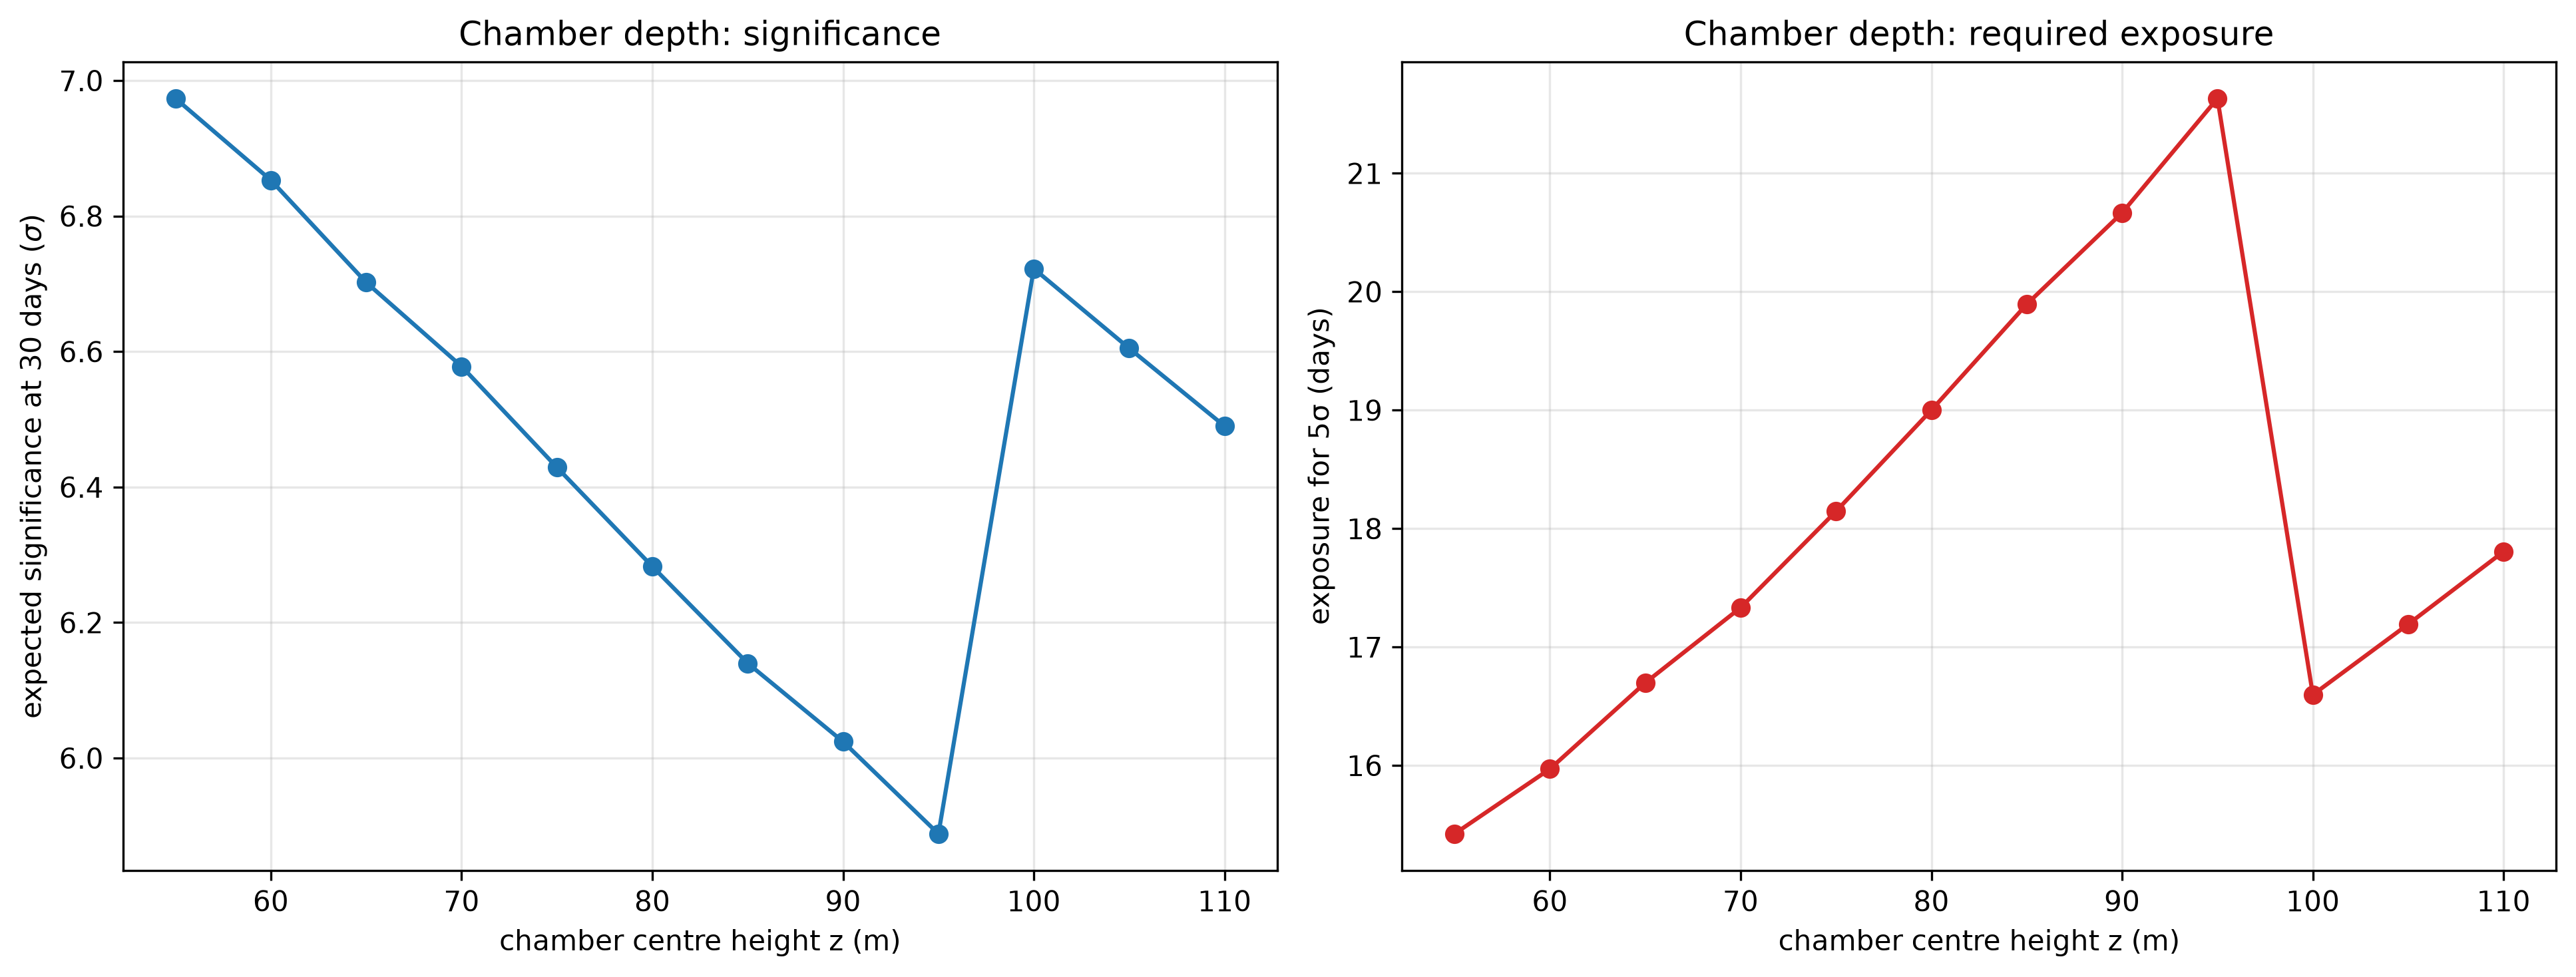
\includegraphics[width=0.49\linewidth]{15_study_B_depth.png}
\end{center}
\spoken
Study A asks how small a chamber we can find. From four to twenty metres the
volume grows by 125, but the significance grows by only a factor nine and the
exposure falls by about seventy. The fit is S proportional to r to the 1.3:
the muon sees the missing chord, about two r, not the volume. Study B asks
whether depth matters. The accessible range is 55 to 110 metres; below about 52
the chamber is outside the field of view. Exposure runs from 15.4 days at 55,
up to 21.6 at 95, then down to 17.8 at 110. Less rock competes with a larger
zenith angle; the rise near the apex is a pyramid geometry effect, not new
physics.
\end{slidebox}

\newpage
\begin{slidebox}{10}{Study C: placement, Study D: binning, and the hill}{1:30}
\onslide
\begin{itemize}
  \item C: best distance $y\approx-25$~m, 15.9 days; baseline 17.3; lateral
        flat within $\pm30$~m.
  \item D: peak $S$ 3.75$\to$18.75 as bins grow 1$^\circ\to5^\circ$; whole
        image stays $\approx3.5\sigma$.
  \item D is a binning study, not a resolution study: no point-spread function.
  \item Malaysian hill: 8~m cave, 9.1 days.
\end{itemize}
\figlabel three figures: C placement, D binning, and the Malaysian hill
density/significance panel; keep the hill smaller.
\begin{center}
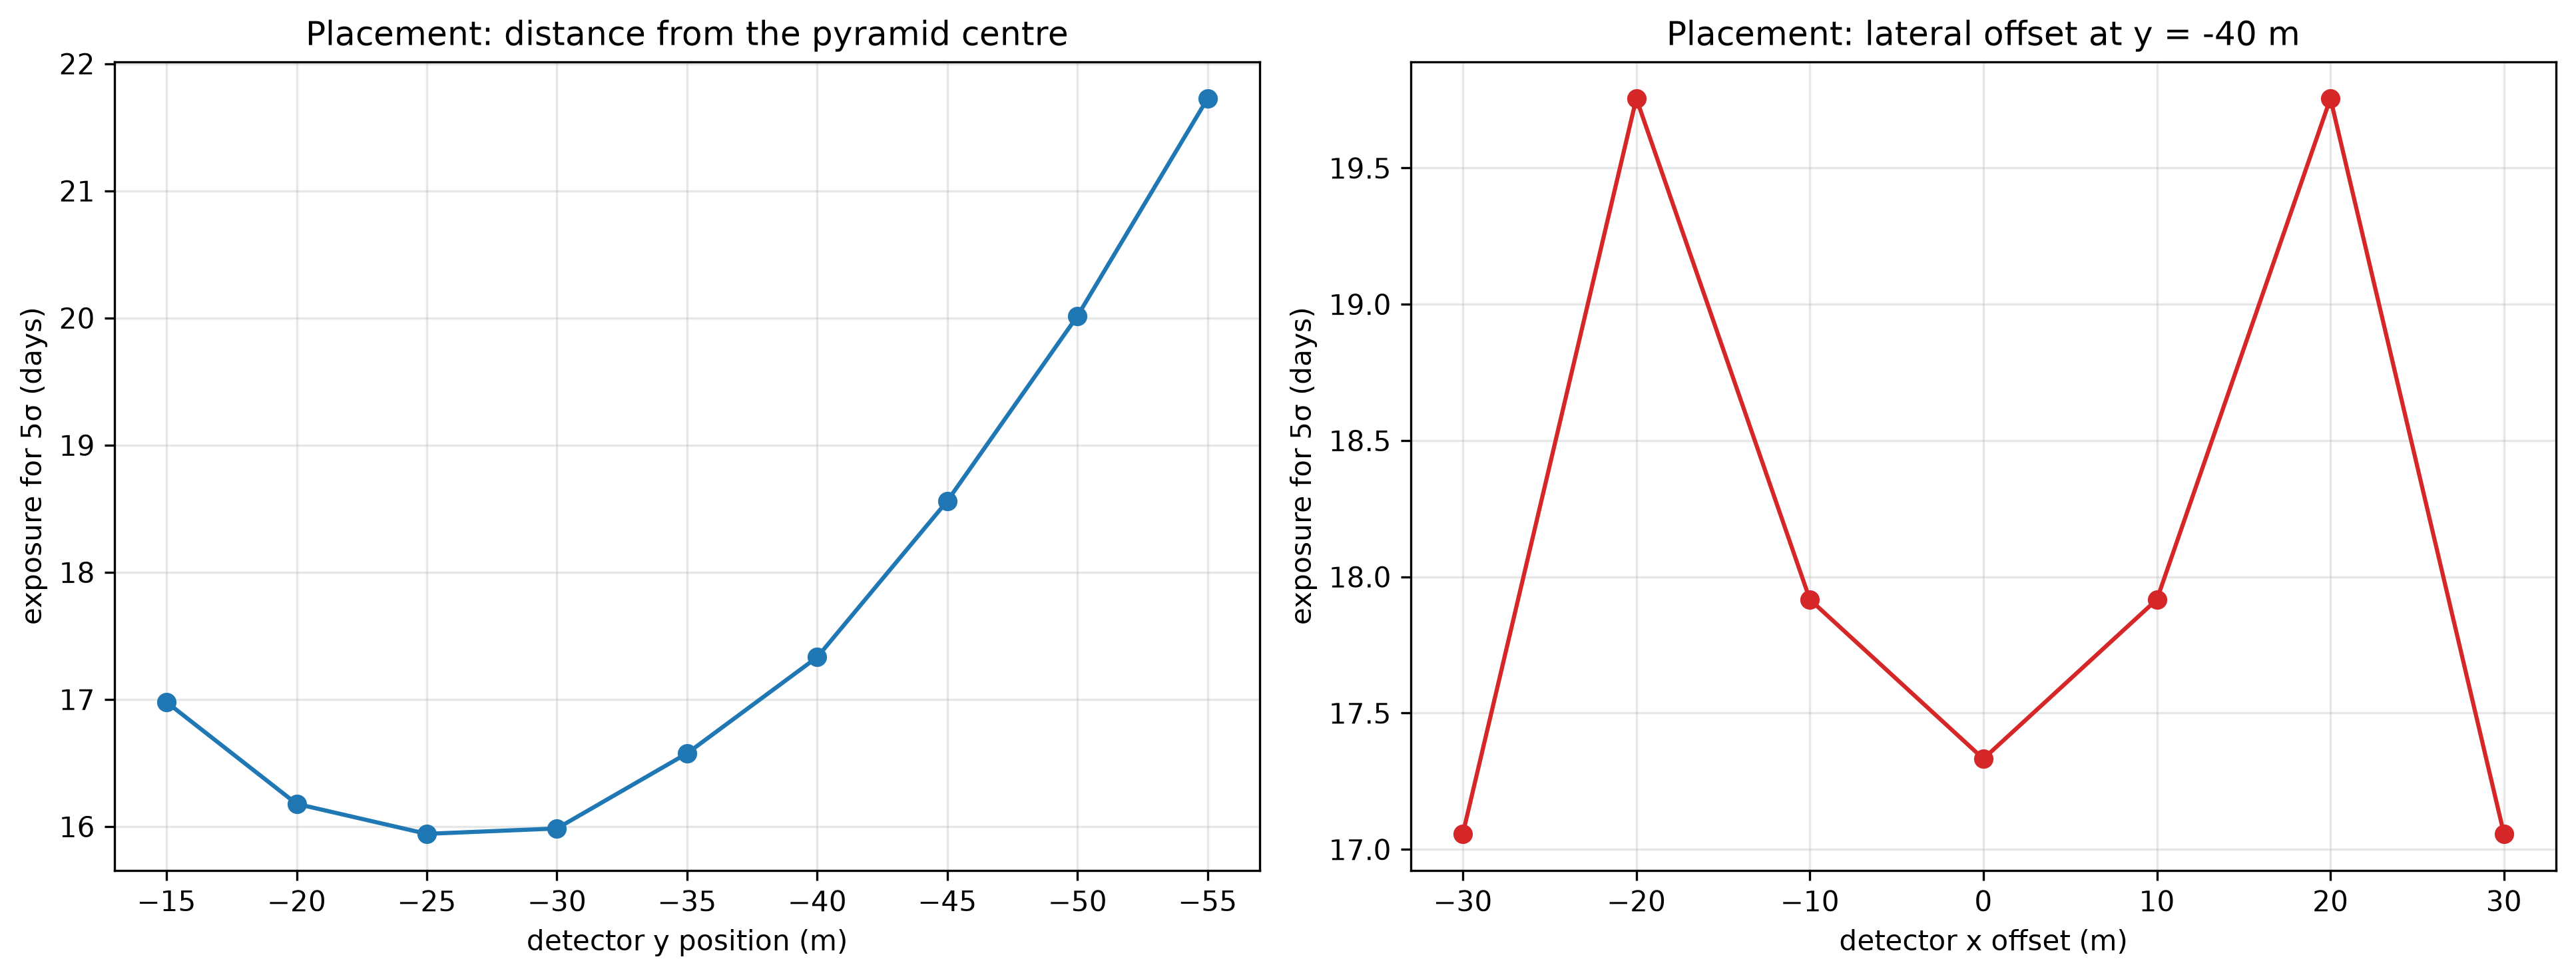
\includegraphics[width=0.33\linewidth]{16_study_C_placement.png}\hfill
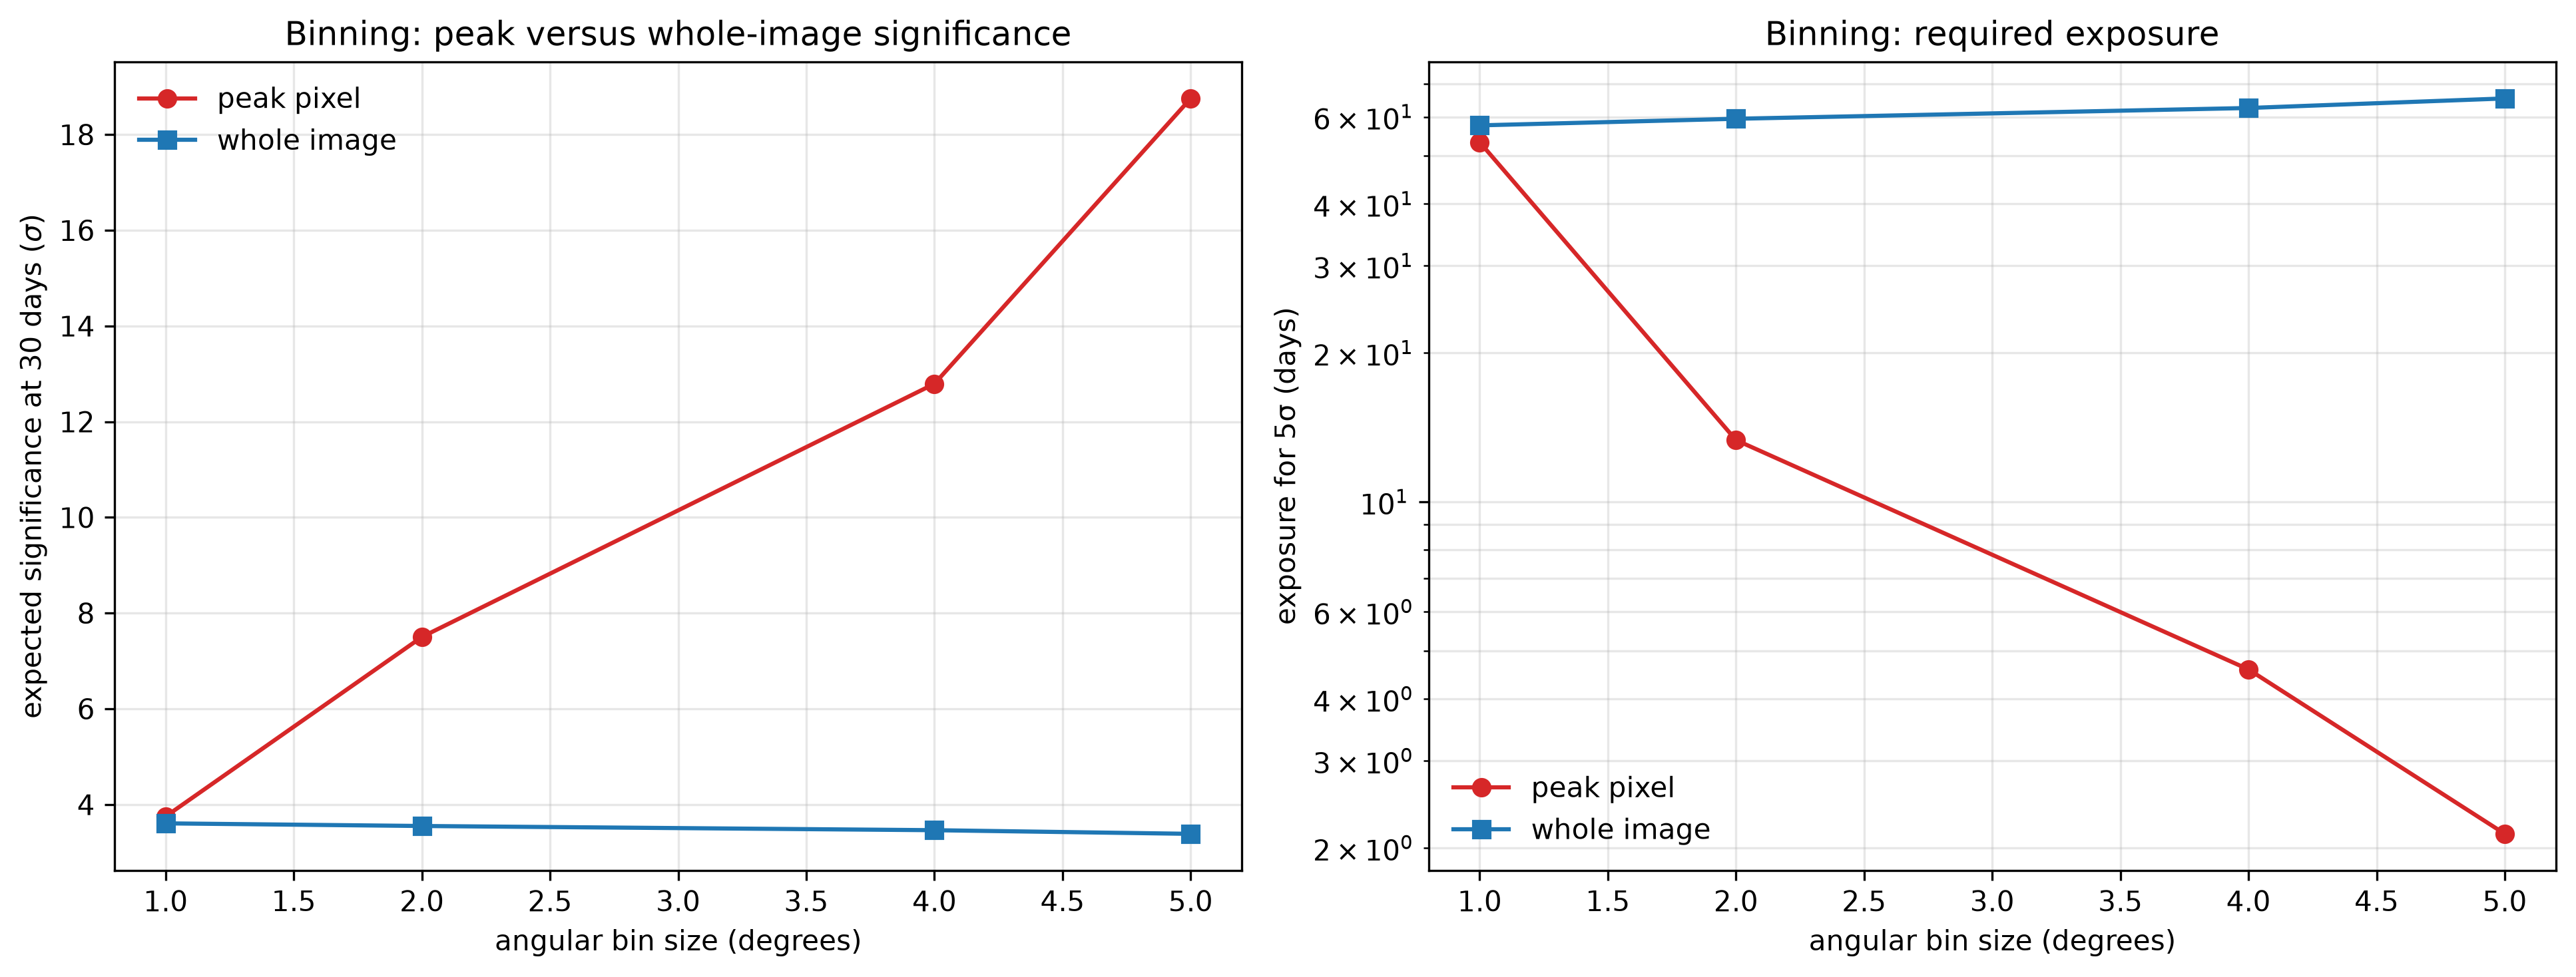
\includegraphics[width=0.33\linewidth]{17_study_D_binning.png}\hfill
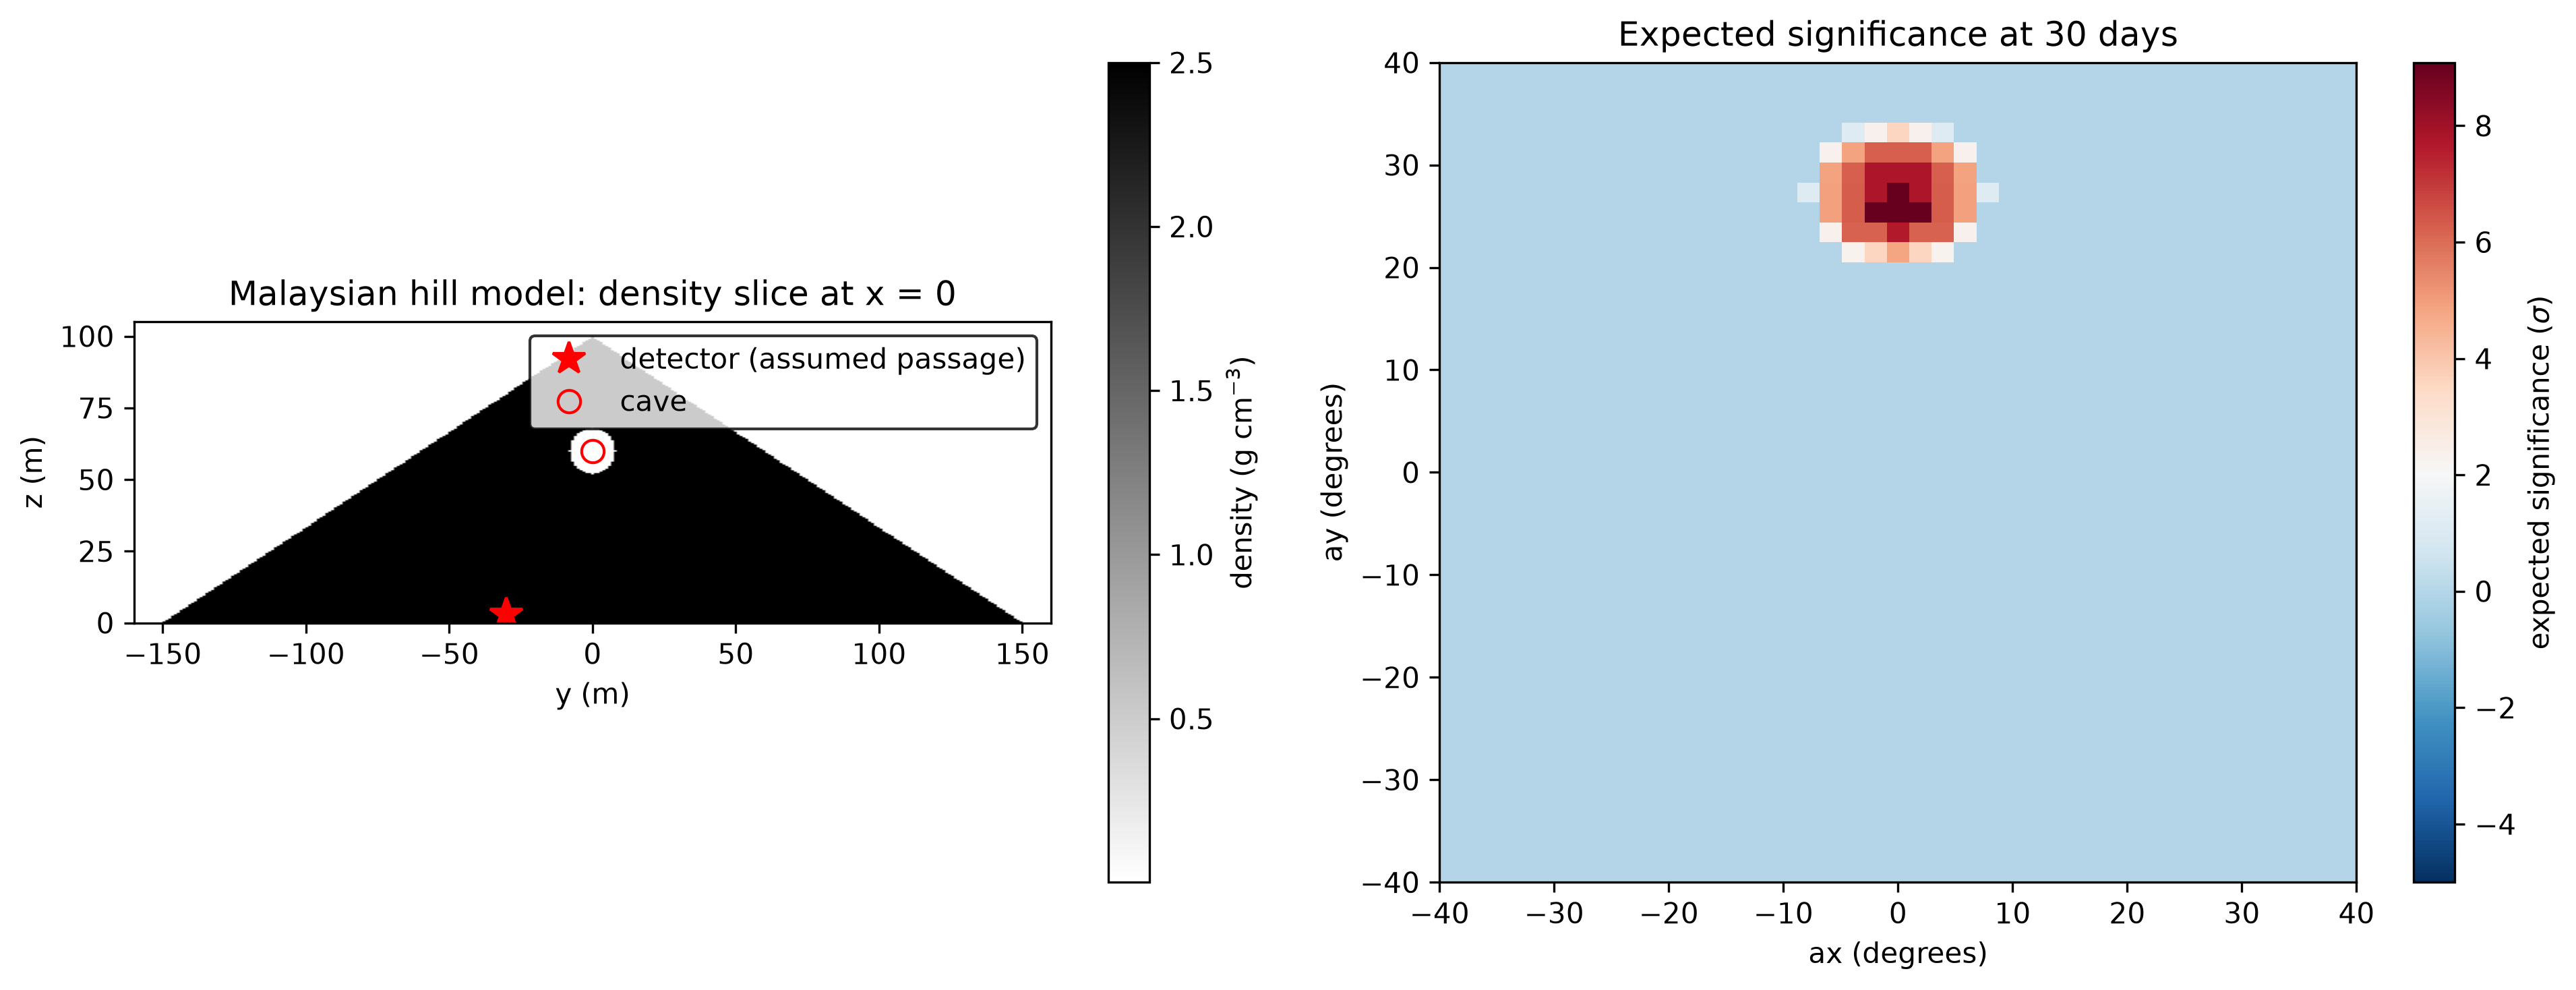
\includegraphics[width=0.28\linewidth]{18_malaysian_target.png}
\end{center}
\spoken
Study C is placement. The distance scan has an optimum near minus 25 metres,
15.9 days, against 17.3 at the baseline and 21.7 at minus 55. The lateral
response is flat within 30 metres. Study D looks like a paradox: peak
significance grows from 3.75 at one degree to 18.75 at five degrees. It is
arithmetic: counts per pixel scale with solid angle, so signal over root
background scales with bin size. The whole-image significance stays at about
3.5 sigma. A real detector would blur neighbouring directions, which we do not
model, so this is a binning study, not a resolution study. Finally, the
hypothetical Malaysian hill with an 8 metre cave needs about 9 days.
\end{slidebox}


\newpage
\begin{slidebox}{11}{Systematics, limitations, and conclusion}{1:30}
\onslide
\begin{itemize}
  \item Density: 4\% error gives fake $3.86\sigma$ at 30 days and
        $9.46\sigma$ at 180 days; the deepest limitation.
  \item Detector efficiency/area: $T_5\propto1/(A\epsilon)$; 50\% efficiency
        doubles exposure.
  \item Missing: scattering, backgrounds, atmospheric variation, real detector
        response, 3D tomography.
  \item Conclusion: 13.4 days for $5\sigma$; geometry and statistics dominate.
\end{itemize}
\figlabel left: density systematics; right: three-pillar TikZ summary
(physics, geometry, statistics) with the headline underneath.
\begin{center}
\begin{minipage}{0.55\linewidth}
\centering
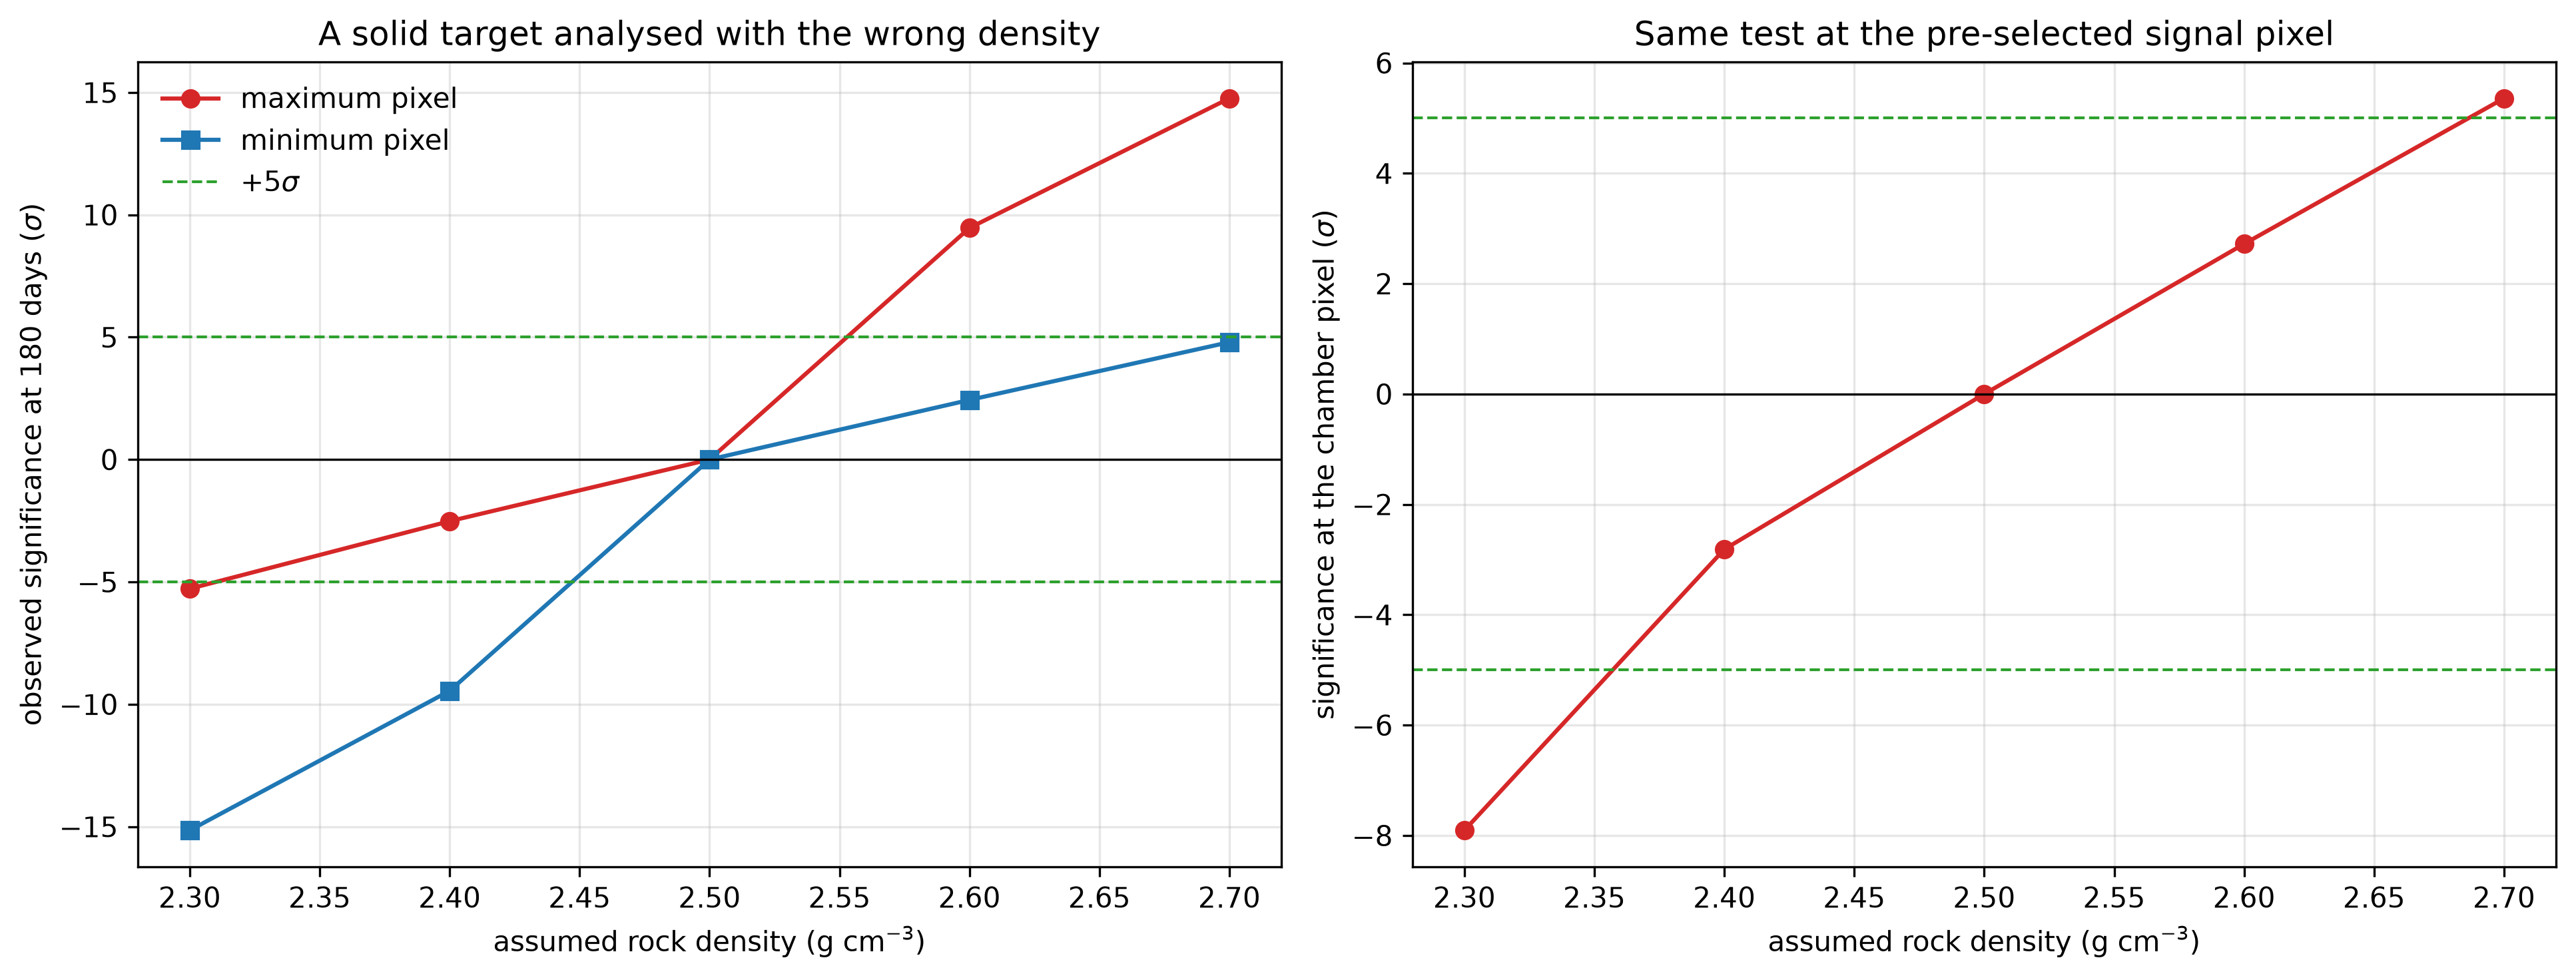
\includegraphics[width=\linewidth]{21_density_systematics.png}
\end{minipage}\hfill
\begin{minipage}{0.42\linewidth}
\centering
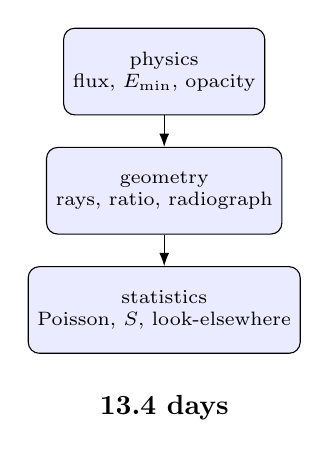
\begin{tikzpicture}[>=Latex,
  pill/.style={draw,rounded corners,fill=blue!8,align=center,
               minimum width=2.5cm,minimum height=1.1cm,font=\scriptsize}]
  \node[pill] (p) {physics\\flux, $E_{\min}$, opacity};
  \node[pill,below=4mm of p] (g) {geometry\\rays, ratio, radiograph};
  \node[pill,below=4mm of g] (s) {statistics\\Poisson, $S$, look-elsewhere};
  \draw[->] (p) -- (g);
  \draw[->] (g) -- (s);
  \node[below=4mm of s,font=\bfseries] {13.4 days};
\end{tikzpicture}
\end{minipage}
\end{center}
\spoken
No result is better than its systematics. The density plot is the important
one: if we assume the rock is four per cent denser than it is, a solid target
produces a fake 3.86 sigma maximum at 30 days and 9.46 at 180, and a fake 2.72
sigma at the chamber pixel. A void and slightly lighter rock are degenerate.
Detector area and efficiency scale the exposure inversely. We do not model
scattering, backgrounds, atmospheric variation, or a real detector response,
and we produce a radiograph, not a 3D inversion. The conclusion is still
13.4 days for five sigma under the stated model, controlled by geometry and
statistics, not by the muon flux alone.
\end{slidebox}

\newpage
\begin{slidebox}{12}{Thank you, references, and Q\&A}{0:30}
\onslide
\begin{itemize}
  \item Thank you. Questions welcome.
  \item Key references used on these slides:
\end{itemize}
\small
\begin{enumerate}[label={[\arabic*]}]
  \item K.~Morishima \textit{et al.}, \textit{Nature} \textbf{552}, 386 (2017).
  \item L.~W.~Alvarez \textit{et al.}, \textit{Science} \textbf{167}, 832 (1970).
  \item G.~Bonomi \textit{et al.}, \textit{Prog.\ Part.\ Nucl.\ Phys.}
        \textbf{112}, 103768 (2020).
  \item Particle Data Group, \textit{Phys.\ Rev.\ D} \textbf{110}, 030001
        (2024).
  \item T.~K.~Gaisser, \textit{Cosmic Rays and Particle Physics} (CUP, 1990).
  \item M.~Guan \textit{et al.}, arXiv:1509.06176 (2015).
\end{enumerate}
\designnote Render this list at 16--18~pt; short-form citations only. The full
bibliography is in the paper.
\figlabel a small TikZ pyramid with the detector and the words
``13.4 days for $5\sigma$'' used as a closing logo.
\begin{center}
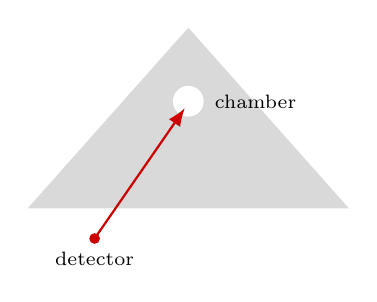
\begin{tikzpicture}[scale=0.85]
  \fill[gray!30] (0,0) -- (2.4,2.7) -- (4.8,0) -- cycle;
  \fill[white] (2.4,1.6) circle (0.23);
  \fill[red!80!black] (1.0,-0.45) circle (0.08);
  \draw[red!80!black,thick,-{Latex}] (1.0,-0.45) -- (2.35,1.5);
  \node[below] at (1.0,-0.5) {\scriptsize detector};
  \node[right] at (2.65,1.6) {\scriptsize chamber};
\end{tikzpicture}
\end{center}
\spoken
Thank you. To summarise: muons give a free, penetrating beam; a twin-target
ratio turns the pyramid into a chamber image; Poisson statistics and the
look-elsewhere effect decide what counts as evidence; and the baseline model
gives 13.4 days for five sigma. The main caveats are the rock density, the
detector response, and the absence of a full 3D inversion. I am happy to take
questions on the method, the numbers, or the limitations.
\end{slidebox}

\end{document}

